\documentclass[12pt,letterpaper,oneside]{scrbook}
\usepackage{lmodern}
\usepackage{amssymb,amsmath}
\usepackage{ifxetex,ifluatex}
\usepackage{fixltx2e} % provides \textsubscript
\ifnum 0\ifxetex 1\fi\ifluatex 1\fi=0 % if pdftex
  \usepackage[T1]{fontenc}
  \usepackage[utf8]{inputenc}
\else % if luatex or xelatex
  \ifxetex
    \usepackage{mathspec}
    \usepackage{xltxtra,xunicode}
  \else
    \usepackage{fontspec}
  \fi
  \defaultfontfeatures{Mapping=tex-text,Scale=MatchLowercase}
  \newcommand{\euro}{€}
\fi
% use upquote if available, for straight quotes in verbatim environments
\IfFileExists{upquote.sty}{\usepackage{upquote}}{}
% use microtype if available
\IfFileExists{microtype.sty}{\usepackage{microtype}}{}
\ifxetex
  \usepackage[setpagesize=false, % page size defined by xetex
              unicode=false, % unicode breaks when used with xetex
              xetex]{hyperref}
\else
  \usepackage[unicode=true]{hyperref}
\fi
\hypersetup{breaklinks=true,
            bookmarks=true,
            pdfauthor={},
            pdftitle={},
            colorlinks=true,
            citecolor=blue,
            urlcolor=blue,
            linkcolor=magenta,
            pdfborder={0 0 0}}
\urlstyle{same}  % don't use monospace font for urls
\setlength{\parindent}{0pt}
\setlength{\parskip}{6pt plus 2pt minus 1pt}
\setlength{\emergencystretch}{3em}  % prevent overfull lines
\setcounter{secnumdepth}{5}

\date{}
\usepackage[top=2.5cm,bottom=2.5cm,left=2.5cm,right=2.5cm]{geometry}
\usepackage[no-math]{fontspec}
\setmainfont{Minion Pro}
%\usepackage{MnSymbol}
%\usepackage[mathlf,textlf]{MinionPro}
\setromanfont{Minion Pro}
\DeclareTextCommand{\nobreakspace}{T1}{\leavevmode\nobreak\ }
\usepackage[spanish, es-tabla]{babel}
\newcommand{\ga}{ɑ}
\usepackage{textcomp}
\usepackage{graphicx}
\graphicspath{{gfx/}}
\usepackage{epstopdf}
\usepackage{acronym}
\usepackage[nouppercase,headsepline,footsepline,plainfootsepline,plainheadsepline]{scrpage2}
\pagestyle{scrheadings}
\clearscrheadfoot
\ohead{\rightmark}
\ihead{\leftmark}
\cfoot{\pagemark}
\automark[section]{chapter}
\newcommand{\subindice}[1]{$_{\text{#1}}$}
\usepackage{mathspec}
\usepackage{amsmath,amsthm}
\usepackage{xltxtra}
\usepackage{tabularx}
\usepackage{titlesec}
\usepackage[usenames,dvipsnames,svgnames]{xcolor}
\usepackage{multirow}
\usepackage{tikz}
\usepackage{tocbibind}
%\renewcommand*\contentsname{Índice}
\renewcommand{\contentsname}{Índice}

\usepackage{pgfplots}
%\pagestyle{plain}
\usepackage{epigraph}
\setlength{\epigraphwidth}{0.7\linewidth}
\setlength{\epigraphrule}{0pt}
\renewcommand*{\textflush}{flushright}
\renewcommand*{\epigraphsize}{\normalsize\itshape}
\newfontfamily\myriad{Myriad Pro}
\newfontfamily\quotefont[Ligatures=TeX]{Myriad Pro}
\titleformat*{\section}{\Huge\myriad}
\titleformat*{\subsection}{\Large\myriad}
\titleformat*{\subsubsection}{\large\myriad}
% Set figure legends and captions to be smaller sized sans serif font
\usepackage[%
    font={small},
    labelfont=bf,
    format=hang,    
    format=plain,
    margin=0pt,
    width=1\textwidth,
]{caption}

\usepackage{subcaption}

%\usepackage[font={footnotesize}]{caption, subcaption}
%\usepackage{subcaption}
\usepackage{siunitx}
	\DeclareSIUnit\molar{{M}}
    \DeclareSIUnit\litro{{L}}
	\DeclareSIUnit\metro{{m}}
	\DeclareSIUnit\gramo{{g}}
% Adjust spacing between lines to 1.5
\usepackage{setspace}
	\onehalfspacing

%\raggedbottom

% Set colour of links to black so that they don't show up when printed
\usepackage{hyperref}
	\hypersetup{colorlinks=true, linkcolor=black}

% Tables
\usepackage{booktabs}
\usepackage{threeparttable}
	\renewcommand{\TPTnoteSettings}{\small
        \setlength\leftmargin{1.8em}%
        \setlength\labelwidth{1em}%
        \setlength\labelsep{.1em}%
		}%
%\usepackage{array}
%\newcolumntype{x}[1]{%
%>{\centering\arraybackslash}m{#1}}%

\begin{document}

\begin{titlepage}
    \begin{center}
    
        %\vspace*{1cm}
        
\includegraphics[width=5cm]{unab}\\
\vspace{0.1cm}
Facultad de Ciencias Biológicas\\
Escuela de Ingeniería en Biotecnología

        \vspace*{1cm}
        
       \large{ \textbf{Modelo molecular en tejido branquial de \emph{Oncorhynchus mykiss} inmunoestimulado con el $\beta$-glucano con \emph{Zymosán A} liberado en dieta}}
        
        \vspace{0.5cm}
        
        \vspace{1.5cm}
 
        Proyecto de tesis presentado como parte de los requisitos para obtener el grado de \\
        \large{\textsc{Magister en Biotecnología}}\\ 
        
        \vspace{2.5cm}        
        presentado por:\\
        \vspace{0.1cm} 
        \textbf{Sebastián Rodrigo Sariego Benítez}\\
        \textbf{Viña del Mar, Chile}
        
       
             
        
         \vspace{1.5cm}
         
    \textbf{Director de Tesis:} Dr. Luis Mercado Vianco\\
       \textbf{Institución:} Pontificia Universidad Católica de Valparaíso
         
       

        
        
 
        Agosto, 2014
        
 
 
     \end{center}
    \thispagestyle{empty}
\end{titlepage}

\clearpage

\frontmatter

\chapter{Resumen}

La perdida del equilibrio
Ambiente\(\Leftrightarrow\)Patógeno\(\Leftrightarrow\)Hospedero es la
causa de la mayoría de las enfermedades presentes en la acuicultura, y
es por eso que es estrictamente necesario cimentar las bases de una
comprensión íntegra del sistema inmune, para así, poder generar
tecnología que pueda sobreponerse a estos paradigmas. Esto tiene suma
importancia sobretodo en la industria acuícola, la cual produce
anualmente, y con un crecimiento constante, 158 millones de toneladas de
pescado, las cuales se traducen aproximadamente en 217.500 millones de
dólares (USD), más aún, de toda esa producción, 136 millones de
toneladas fueron exclusivamente destinadas a consumo humano. Esto
demuestra el potencial presente en esta industria, industria que se ve
año a año afectada por la mortalidad de las distintas especies por la
perdida del equilibrio antes mencionado, generándose cuantiosas perdidas
a nivel comercial y de capital humano.

Los inmunoestimulantes han surgido como una opción viable, escalable y
económica para solventar parte de los problemas de la acuicultura,
fortaleciendo la capacidad de respuesta inmune de los organismos
cultivados en distintos estadíos de desarrollo. Dentro de las formas en
las cuales se pueden desplegar estos inmunoestimulantes podemos
encontrar vacunas, suspensión oral y liberación en el alimento, entre
otras.

En este estudio se utilizó una dieta en base a harina de pescado y otros
nutrientes con la cualidad de contener Zimosán A para ser liberado en la
alimentación de especímenes de Trucha arcoiris. Durante 28 días de
tratamiento se generaron muestreos de branquias, para así, evaluar la
capacidad de respuesta inmune que levanta el organismo frente a la
suplementación de este inmunoestimulante en su dieta. La respuesta se
midió en base a distintos marcadores, reguladores y efectores de la
inmunidad, a nivel de expresión y de disponibilidad de estos. Por estar
involucrados en la primera fase de respuesta inmune los marcadores
seleccionados a estudiar fueron: El factor de necrosis tumoral alfa,
interferón gamma, interleuquinas 1 beta y 12, y finalmente la enzima
oxido nítrico sintasa de carácter inducible. Mediante ensayos de PCR en
tiempo real se pudo evaluar que la respuesta frente a la inducción por
este \(\beta\)-glucano empieza a levantarse pasado el día 14 del
tratamiento, teniendo en común estas fechas para todos los marcadores
evaluados.

Para evaluar la disponibilidad de estas moléculas se utilizaron dos
alcances, uno a nivel de ELISA, ensayo en el cual pudimos obtener
resultados de aumento de disponibilidad entre los días 21 y 28 de
muestreo; y a nivel de inmunohistoquímica de fluorescencia, teniendo en
cuenta los días elevados mostrados por el ensayo anterior, se pudieron
observar marcajes de las distintas moléculas estudiadas en muestras de
tejido branquial.

\chapter{Abstract}

The loss of balance between
Environment\(\Leftrightarrow\)Pathogen\(\Leftrightarrow\)Host is one of
the main causes of the most of diseases presents in the global
aquaculture, and that is why it's absolutely necessary to cement the
foundation for a comprehensive understanding of the immune system, thus,
to generate technology that can overcome these paradigms. This is
especially important in the aquaculture industry, which produces
annually, and with steady growth, 158 million tons of fish, which
translates into approximately 217,500 million dollars, even more, of all
that production, 136 million tons were used exclusively for human
consumption. This demonstrates the potential in this industry, an
industry that is affected by mortality of different species every year,
by the loss of the aforementioned balance, generating substantial losses
in commercial and human capital.

Immunostimulants have emerged as viable, scalable and economical option
to solve in part the problems of aquaculture, strengthening the immune
responsiveness of farmed species at different stages of development.
Among the ways in whic they can deploy these immunostimulants we find
vaccines, oral suspension and food release, among others.

In this study we used a diet based on fish meal and other nutrients,
supplemented with Zymosán A (0,3\%) to be released in the feeding of
rainbow trout specimens. During 28 days of treatment, gills were taken
in order to evaluate the ability of immune response that raises the
organism facing this immunostimulant supplementation in their diet. The
response was measured based on different markers, regulators and
effectors of immunity, at expression and bioavailability levels.

Being involved at the first stage of immune response, selected markers
sudied were: tumor necrosis factor alpha, interferon gamma, interleukin
1-beta and 12, and finally the inducible nitric oxide synthase. Through
real-time PCR assays could be assessed that the response to this
induction with this \(\beta\)-glucan begins to rise past the 14th day of
treatment, having in common these days for all the tested markers.

To evaluate the bioavailability of these molecules we've used two
scopes, using ELISA assay in which we get results from increased
bioavailability between 21 and 28 days, and, immunohistochemistry with
fluorescence, considering the high days displayed by the ELISA results
was possible to observe the different studied moleculas in gills tissue
samples. \tableofcontents
\clearpage
\cleardoublepage
\chapter{Lista de abreviaturas}

\begin{acronym}
    \acro{fao}[FAO]{\emph{Food and Agriculture Organization of the United Nations}, Organización de las Naciones Unidas para la Alimentación y la Agricultura}
    \acro{ciac}[CIAC]{Centro de Investigacíones en Acuicultura Curauma}
    \acro{bsa}[BSA]{\emph{Bovine albumine serum}, Albúmina de suero bovino}
    \acro{dna}[DNA]{\emph{Deoxyribonucleic Acid}, Ácido desoxirribonucleico}
    \acro{cdna}[cDNA]{DNA complementario}
    \acro{rna}[RNA]{\emph{Ribonucleic Acid}, Ácido ribonucleico}
    \acro{pcr}[PCR]{\emph{Polimerase Chain Reaction}, Reacción en cadena de la polimerasa}
    \acro{qpcr}[qPCR]{\emph{(semi)Quantitative PCR}}, PCR Cuantitativa
    \acro{ifat}[IFAT]{\emph{Immunofluorescence antibody test}, Prueba de inmunofluorescencia con anticuerpos}
    \acro{elisa}[ELISA]{\emph{Enzyme linked immuno-sorbent assay}, Ensayo de inmunoabsorción ligado a enzimas}
    \acro{sdspage}[SDS-PAGE]{\emph{SDS-Polyacrilamide gel electrophoresis}}
    \acro{mq}[MQ]{\emph{Milli-q}}
    \acro{sds}[SDS]{\emph{Sodium dodecyl sulfate}, Dodecil sulfato de sodio}
    \acro{tmb}[TMB]{3,3'-5,5'-tetrametillbencidine}
    \acro{gialt}[GIALT]{\emph{Gill associated lymphoid tissue}, Tejido linfoide asociado a branquias}
    \acro{rt}[RT]{Retrotranscripción}
    \acro{om}[OM]{\emph{Oncorhynchus mykiss}}
    \acro{il}[IL]{Interleuquina}
    \acro{il1b}[IL-1$\beta$]{Interleuquina 1-beta}
    \acro{il12}[IL-12]{Interleuquina 12}
    \acro{ifng}[IFN-$\gamma$]{Interferón gama}
    \acro{tnfa}[TNF-$\alpha$]{Factor de necrosis tumoral alfa}
    \acro{pbs}[PBS]{\emph{Phosphate Buffered Saline}, Tampón fosfato salino}
    \end{acronym}

\clearpage
\listoffigures
\cleardoublepage
\listoftables

\mainmatter
\chapter{Introducción}\label{cap.introduccion}

Las primeras truchas en Chile fueron introducidas a fines del siglo XIX,
específicamente en 1880 en la actual región del Bio-Bio. Las primeras
ovas introducidas fueron las de la llamada ``trucha común'', actualmente
conocida como trucha fario (\emph{Salmo trutta}). No fue hasta en la
primera década del siglo XX que el gobierno de ésa época, respondiendo a
las inquietudes de un naturalista alemán llamado Federico Albert, quien
había realizado un catastro de las posibles especies de salmónidos que
podrían ser introducidos en nuestro país, el cual reconoce el potencial
poder económico de estos salmónidos e introduce, junto a la creación de
la Piscicultura Río Blanco, tres especies traídas desde Francia, la
Trucha Fario, la Trucha arcoiris (\emph{Oncorhynchus mykiss}) y el
Salmón del atlántico (\emph{Salmo salar}).

\section{El género \emph{Oncorhynchus}}

Onchorhyncus corresponde a uno de los 10 géneros de la familia
Salmonidae y tiene alrededor de 12 especies, incluyendo \emph{O.mykiss}
(trucha arcoiris), \emph{O. nerka} (salmón rojo), \emph{O. gorbuscha}
(salmón rosado), \emph{O. tshawytscha} (salmón chinook),
\emph{O. kisutch} (salmón coho) , entre otros. Se distribuyen principal
y naturalmente por una vasta zona que comprende desde California hasta
el mar de Behring y el océano ártico (C. Groot y Margolis, 1991).

Algunas características principales de este género son las siguientes

\begin{itemize}
    \item Son peces anádromos, es decir emigran al mar cuando son juveniles y luego vuelven al agua dulce para reproducirse.
    \item A su vez, en su mayoría solo se reproducen una vez, por lo tanto son semélparos.
    \item Tienen baja tasa de fecundidad (2 a 5mil ovas) y grandes huevos (5-8mm)
\end{itemize}

En Chile encontramos la trucha arcoiris, el salmón coho
(\emph{Oncorhynchus kisutch}) y el salmón chinook
(\emph{Oncorhynchus tshawytscha}) como representantes de este género.

La trucha arcoiris, descrita inicialmente por Walbaum en 1972 tiene un
cuerpo alargado fusiforme con 60 a 66 vértebras, con 3 a 4 espinas
dorsales, 10 a 12 rayos dorsales blandos, 3 a 4 espinas anales, 8 a 12
rayos anales blandos y 19 rayos caudales. Presentan una aleta con gran
tejido adiposo, la cual usualmente contiene un borde negro. Tienen como
coloración principal tonalidades de azul a verde oliva, sobre una banda
rosa a lo largo de la linea lateral y plateada por debajo de ella,
configuración cromática que le da su nombre \emph{arcoiris}.

\begin{figure}[h!]
    \centering
    \includegraphics[width=15cm]{1} 
    \caption {Ciclo productivo de la trucha arcoiris}
    \label {fig:ciclo}
\end{figure}

Este pez es resistente, de crecimiento rápido y tolerante a una amplia
gama de manipulaciones y ambientes, pudiendo así ocupar una variedad de
hábitats y diferentes temperaturas. La temperatura ideal para el cultivo
de la trucha arcoiris está por debajo de 21º C, aunque en etapa de
desove y crecimiento la temperatura tiene que estar en el rango de 9 a
14ºC (Figura \ref{fig:ciclo}).

\subsection{Situación actual en Chile}

Los desembarques de Trucha arcoiris han aumentado cercano al 1500\% en
20 años (Figura \ref{desembarques}), con una tasa de crecimiento
porcentual promedio del alrededor del 15\% (Sernapesca, 2012), en
términos monetarios, el año 2013 la exportación de este producto generó
ventas alrededor de los 300 millones de dólares, lo que lo convierte en
una de las 3 especies más cosechadas en Chile junto al Chorito y el
Salmón del atlántico (Subpesca, 2013).

\begin{figure}[h]
    \centering
    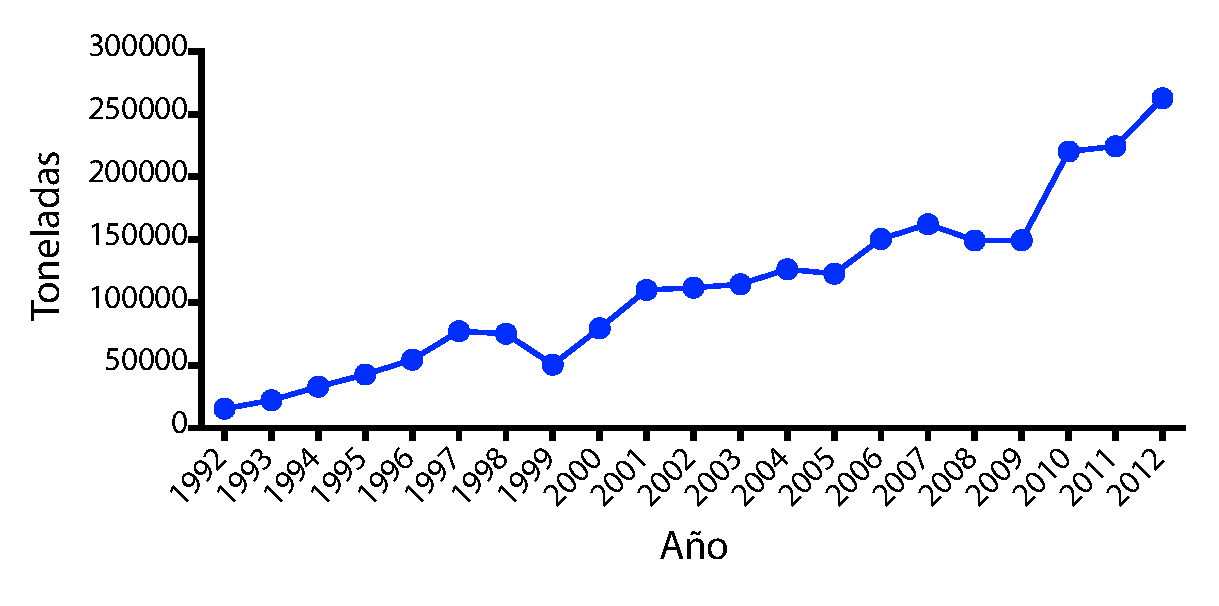
\includegraphics[width=0.9\textwidth]{desembarques.eps}
    \caption{Desembarques de Trucha arcoiris en Chile} \label{desembarques}
\end{figure}

Los sistemas de cultivo, debido al crecimiento acelerado de la
producción enfrentan diferentes problemas, por una parte patógenos como
\emph{Flavobacterium psychrophilum} y \emph{Piscirickettsia salmonis},
llegando a haber muertes en casos de hasta el 50\% y 34\% de la
producción respectivamente. La explicación de esto radica en la pérdida
del equilibrio ambiente-patógeno-hospedero, lo cual genera las
condiciones que hacen aumentar la enfermedad y mortalidad en el cultivo;
y por otra parte el estrés en que se ven sometidos los organismos
(Georgiadis et~al., 2001; FAO, 2012). Estas enfermedades, cualquiera sea
su origen, pueden tener un alto impacto negativo en la producción
mundial, lo que equivale a grandes pérdidas económicas (Z. J. Shao,
2001). Para comprender y crear soluciones se requiere conocer aspectos
fundamentales de la defensa, especialmente del sistema inmune.

\section{Sistema inmune en peces}

La comprensión de la funcionalidad del sistema inmune de peces,
especialmente en teleósteos, al igual que en vertebrados superiores se
puede entender como una respuesta innata o inespecífica y una respuesta
adaptativa o especifica (Olabuenaga, 2000; Fernández et~al., 2002).

La respuesta inmune innata o inespecífica en peces es muy importante, ya
que constituye la primera y más importante línea de defensa del pez
frente a un gran número de patógenos, en esta respuesta convergen
factores humorales y celulares (Olabuenaga, 2000; Fernández et~al.,
2002; L.-Y. Zhu et~al., 2012). Este tipo de inmunidad está basado en el
reconocimiento no clonal de los componentes estructurales o secretados
de los patógenos microbianos (Athman y Philpott, 2004), los cuales son
llamados patrones moleculares asociados a patógenos (o PAMPs, por sus
siglas en inglés), estos a su vez son reconocidos por receptores de
reconocimiento de patrón (PRR, por sus siglas en inglés) (Gordon, 2002),
entre los cuales se encuentran receptores de tipo Toll (TLR, por sus
siglas en inglés), el receptor de complemento tipo-3 (CR3), Dectina-1,
proteína C-reactiva, entre otros (Rondon-Barragan, 2010). Entre los
PAMPs más clásicos se puede encontrar a las secuencias de ADN CpG sin
metilar, los lipopolisacáridos (LPS) y el RNA bicatenario viral. La
interacción entre los PRR (como los TLR) y los PAMP es la reacción que
desencadenará e iniciará la transducción de señales intracelular que
resultara en la expresión de genes involucrados en la inflamación,
respuesta antiviral y maduración de células con fenotipo dendrítico
(Aghaallaei et~al., 2010); TLRs individuales activan factores de
transcripción únicos y comunes a través de diferentes vías de
señalización para generar una respuesta biológica especifica ante
microorganismos (N. C. Bols et~al., 2001; A. E. Ellis, 2001; Kawai y
Akira, 2005)

Entre las células involucradas la fase celular inespecífica de la
respuesta inmune están las células citotóxicas no específicas (NCC, por
sus siglas en inglés), células fagocíticas, y granulocitos (A. E. Ellis,
1977; Ainsworth, 1992). Las células NCC en peces se encuentran
principalmente en el riñón cefálico, el bazo, sangre periférica y el
timo, son células citotóxicas inespecíficas, es decir ejercen su acción
en diferentes células diana sin un reconocimiento previo, las cuales
requieren un contacto célula-célula para poder efectuar la lisis celular
(Graves et~al., 1984). Dentro de las células fagocíticas los neutrófilos
representan aproximadamente en promedio a un 11\% de los leucocitos en
sangre, son también llamados polimorfonucleares o leucocitos
específicos, su capacidad fagocítica es baja, ya que ingieren poco
material extraño, aunque poseen la mayoría de la batería enzimática para
este trabajo. Los eosinófilos y basófilos son los granulocitos con menor
presencia en peces, aunque en el caso de los eosinófilos se han logrado
encontrar en peritoneo u otros tejidos como el intestino, mientras que
los basófilos tienen escasa presencia en estos organismos (D. Palić
et~al., 2011).

Dentro del sistema fagocítico mononuclear, podemos encontrar a los
monocitos y a los macrófagos (derivados de estas últimas), los primeros
son móviles y generalmente más grandes que los demás leucocitos, en el
caso de los macrófagos, pueden fagocitar partículas mucho más grandes,
son abundantes en el bazo y riñón cefálico, aunque también se han
encontrado en mucosa olfatoria (Olabuenaga, 2000; R Castro et~al.,
2011).

Entre los componentes moleculares asociados a la respuesta innata del
sistema inmune de peces podemos encontrar a las citoquinas, las cuales
son una familia de proteínas de bajo peso molecular (comúnmente
glicosiladas) y secretadas por células del sistema inmune activadas
previamente frente a la exposición de diferentes componentes patógenos
(Salazar-Mather y Hokeness, 2006)⁠. Estas citoquinas pueden dividirse en
interferones (IFNs), interleuquinas (ILs), factores de necrosis
tumorales (TNFs, por sus siglas en inglés), factores estimuladores de
colonias y quimioquinas (Savan y Sakai, 2006)⁠. Las interleuquinas son
citoquinas producidas principalmente por linfocitos T CD4+, aunque
también son secretadas por una gran variedad de tipos celulares, como
por ejemplo los macrófagos/monocitos y las células endoteliales (C. J.
Secombes et~al., 2011), las quimioquinas, o también llamadas citoquinas
quimiotácticas (o quimioatractantes) son una familia de citoquinas que
son liberadas por la mayoría de tejidos infectados en los estadíos
tempranos de infección. Las citoquinas pueden dividirse en distintas
familias según sea la organización de sus cisteínas.

Dentro de la familia de las interleuquinas podemos encontrar la
Interleuquina 1 \(\beta\), la citoquina proinflamatoria mas estudiada,
todo debido a su rol mediador de enfermedades autoinflamatorias. Es
producida principalmente por macrófagos activados, celulas dendríticas y
monocitos, y afecta a casi cualquier tipo celular, jugando un rol
central en la generación de respuestas sistémicas y locales a la
infección, asi como también en respuesta a daños y desafíos
inmunológicos (Reis et~al., 2012). Esta citoquina potencialmente induce
la proliferación, diferenciación y activación de celulas no específicas,
como NK, macrofagos, etc\ldots{}, así como también una respuesta inmune
específica, activando linfocitos B y T (Hong et~al., 2004;
Taechavasonyoo et~al., 2013). Junto con IL-1\(\beta\) existe otro
marcador que sirve para evaluar si es que los inmunoestimulantes inducen
o no una respuesta inflamatoria, este otro marcador es el Factor de
necrosis tumoral (TNF-\(\alpha\)). este factor tiene una variedad de
funciones inmunológicas, regulando la inflamación y la respuesta inmune
celular(J. Zou et~al., 2003; T. Wang et~al., 2004; Teles et~al., 2011).
Promueve la necrósis hemorrágica de tumores, así como también mejora la
fagocitosis y citotoxicidad de neutrofilos. Mejora la sintesis de
prostaglandina E2 y oxido nítrico (NO), y modula la expresión de muchas
citoquinas, incluyendo IL-1, IL-6 y algunas quimioquinas. IL-1\(\beta\)
y TNF-\(\alpha\) son ampliamente usados como marcadores de respuesta
inmune innata (Z. Zhang et~al., 2009).

Otra citoquina importante en el proceso inmunitario es Interferón Gamma
(IFN-\(\gamma\)), perteneciente a la familia de los Interferones,
moleculas encargadas principalmente en la respuesta viral, aunque
también son importantes reguladores del sistema inmunitario innato y
adaptativo (Savan y Sakai, 2006). El IFN-\(\gamma\) es producido en una
primera etapa por celulas NK estimuladas por las interleuquinas 12 y 18,
las cuales son producidas por fagocitos mononucleares y celulas
presentadoras de antígenos (APCs, por sus siglas en inglés). Al ser
secretada esta molécula se une a su receptor y por la via Jak/STAT
promueve la activación de macrófagos aumentando la sintesis de la
fagocito oxidasa dependiente de NADPH (\si{gp91^{phox}} y
\si{p67^{phox}}), la oxido nítrico sintasa 2 (NOS2), p47 GTP-asa y la
proteina de union a guanilato, así como también aumenta las moleculas de
MHC de clase 2 en macrofagos y otras APCs (U. Boehm et~al., 1997). Por
lo tanto en contraste con los interferones de tipo I
(IFN-\(\alpha\)/\(\beta\)) el IFN-\(\gamma\) juega un rol clave en la
activación de macrofagos para aumentar destrucción de patógenos
bacterianos, protozoos y virales (Fields et~al., 2007).

La interleuquina 12 (IL-12) es una citoquina heterodimérica, compuesta
por la subunidades P35 y P40, la primera miembro de la familia de la
interleuquina 6 con 4 \(\alpha\)-helices en su topología y p40 recuerda
una forma asociada a un receptor de citoquinas solubles(Yoshiura et~al.,
2003; Huising et~al., 2006). Esta citoquina pro-inflamatoria es
producida en las etapas iniciales de la respuesta inmune por monocitos,
macrófagos, celulas dendríticas y neutrofilos, y una de sus principales
funciones es inducir la sintesis de otras citoquinas, como el
anteriormente nombrado IFN-\(\gamma\), que sirve como orquestador en la
maduración de un linfocito T \emph{naive} a un fenotipo Th1 (Nascimento
et~al., 2007), y es gracias a esta función se considera como un
medidador entre la respuesta innata y adaptativa de la inmunidad (Lu
Zhang et~al., 2014).

Dentro de las moleculas efectoras de la respuesta inmune la oxido
nítrico sintasa de tipo inducible (iNOS), propia de fagocitos (Wu
et~al., 2008; Zhao et~al., 2010), aumenta su expresión durante eventos
de inflamación, y a su vez, es propia del estallido respiratorio de los
macrófagos proveyendo así a la celula de un ambiente citotóxico ideal
para los eventos pro-inflamatorios por la producción de Oxido Nítrico
(NO), catalizando la oxídación de L-arginina (Yang et~al., 2013). Esta
molecula, puede ser activada en monocitos, macrófagos, células
dendríticas, neutrofilos y células NK ya sea por citoquinas,
endotoxinas, o ambas (MacMicking et~al., 1997; Bogdan, 2001). estas
características demuestran la importancia del rol de iNOS y su producto
gaseoso NO en el sistema inmune, ya que a diferencia de las otras NOS,
la neuronal (nNOS) y la endotelial (eNOS) esta no tiene una sintesis
basal ni constitutiva, haciendo de esta molecula un marcador
inmunológico de importancia para estudiar procesos inmunológicos.

Otras moléculas efectoras presentes en la respuesta innata frente a
patógenos son los péptidos anti-microbianos (AMP, por sus siglas en
inglés), moléculas con la capacidad de destruir y/o neutralizar
microorganismos patógenos directamente, son moléculas pequeñas,
anfipáticas y catiónicas (L. Mercado et~al., 2005), y están ampliamente
extendidos por los reinos vegetal y animales (Zasloff, 2002). Los
mecanismos de acción anti-bacteriana de estos AMP pueden entenderse
desde dos puntos de vista diferentes: 1. La estructura anfipática puede
unirse selectivamente a la membrana bacteriana y generar poros
transmembrana, los cuales destruyen a la bacteria desintegrando la
membrana, y 2, los AMP pueden directamente entrar a la bacteria e
interactuar específicamente con factores de crecimiento y metabolismo
bacteriano eventualmente generando la muerte bacteriana (Wimley, 2010;
L.-Y. Zhu et~al., 2012). Entre los péptidos anti microbianos descritos
en peces podemos encontrar cuatro grandes grupos, las defensinas,
proteínas de macrófagos asociadas a resistencia natural (Pramps, por sus
siglas en inglés), NK-lisina y hepcidinas.

Otra familia de péptidos antimicrobianos son las Catelicidinas,
presentes generalmente en neutrófilos y superficies de mucosas, su
actividad se centra principalmente en su interacción con la membrana
plasmática de la bacteria para eventualmente destruirla, fueron
primeramente descritas en mamíferos y luego se han encontrado en
distintos peces teleósteos, algunos casos son los de trucha arcoíris
(C.-i. Chang et~al., 2005), bacalao (Maier et~al., 2008), salmón del
atlántico (C.-I. Chang et~al., 2006), entre otras.

Además de poseer una estructurada y bien desarrollada respuesta inmune
innata como se explicaba anteriormente, los peces también cuentan con
una respuesta adaptativa, con componentes celulares y humorales
(Alvarez-Pellitero, 2008), en este último grupo se encuentran los
anticuerpos, los cuales son proteínas pertenecientes al grupo de las
inmunoglobulinas (Ig), en el caso de los peces producen inmunoglobulinas
del tipo M, T y D (Bengtén et~al., 2002; Ling Zhang et~al., 2011; L.-Y.
Zhu et~al., 2012), siendo la primera la más importante, estando presente
en el suero, el mucus y la bilis. Los anticuerpos son producidos por
linfocitos B activados al reconocer algún antígeno, ya sea en solución o
presentado por alguna célula presentadora de antígeno, que en el caso de
los peces principalmente son macrófagos, y tienen variadas funciones,
pueden actuar como moléculas efectoras en el suero, o también como
receptores de superficie de linfocitos B.

Una de las principales diferencias entre el sistema inmune de peces
teleósteos con el de mamíferos es la carencia de medula ósea y ganglios
linfáticos, por lo cual no se puede marcar una diferencia entre órganos
hematopoyéticos y órganos linfoides (Olabuenaga, 2000; Fernández et~al.,
2002). Entre los principales órganos pertenecientes al sistema inmune de
peces podemos encontrar el timo, el riñón y el bazo. El riñón cefálico
es el principal órgano en la diferenciación de linfocitos B, ya que es
el primer órgano en el que aparecen estas células durante el desarrollo
del pez, también es el órgano donde se produce la eritropoyesis,
granulopoyesis, linfopoyesis y monocitopoyesis (Whyte, 2007), por lo que
se le puede considerar a la vez un órgano análogo a la medula ósea de
los mamíferos (Razquin et~al., 1990). Los centros melanomacrofágicos son
una agregación de macrófagos que contienen melanina, un pigmento de
color oscuro, su tamaño y número está directamente relacionado con el
estado del pez, ya que estas variables aumentan considerablemente en
peces enfermos, donde el catabolismo ha sido excesivo. Algunos estudios
ontogénicos realizados en salmónidos sugieren que la función del bazo no
es esencial en la maduración del sistema inmunológico, ya que los
linfocitos del timo y riñón cefálico estarían más involucrados que este
órgano en esta maduración. Otros estudios sin embargo indican, que bajo
un desafío antigénico aparecen linfocitos B en el bazo, teniendo
parámetros similares a los presentados por estas células en otros
órganos como el riñón cefálico.

\section{Inmunidad en mucosas}

La mayoría de las infecciones empiezan o afectan las mucosas epiteliales
de los animales. El campo de la investigación en inmunología de mucosas
ha crecido sin precedentes durante los últimos años, así como también
nuestro conocimiento en la materia, específicamente como las superficies
de las mucosas responden a los variados antígenos que constantemente
invaden estos tejidos. En teleósteos los principales tejidos con
mucosas, y por ende las primeras mas accesibles barreras inmunológicas
son el intestino, la piel y las branquias (Gomez et~al., 2013). El
intestino, la piel y las branquias contienen tejido linfóide asociado a
mucosa (MALT, por sus siglas en inglés) que tiene un rol fundamental en
el mantenimiento de la homeostasis en la mucosa. Este tejido linfoide
asociado a mucosa está dividido en tejidos linfoides asociados a
intestino, piel y branquias (GALT, SALT y GIALT, respectivamente, por
sus siglas en inglés). Estas superficies mucosas están cubiertas por una
capa protectora de mucus rico en factores inmunológicos, como las
lectinas, mucinas, peptidos antimicrobianos, toxinas e inmunoglobulinas
(Lazado y Caipang, 2014).

\begin{figure}[h!]
    \centering
    \includegraphics[width=\textwidth]{mucosalimmunity} 
    \caption {Representación esquemática de las similitudes y diferencias entre las superficies mucosas de teleósteos como piel, intestino y branquias y de mamiferos como piel y mucosa de tipo 1. Adaptado y traducido desde ``The mucosal immune system of fish: The evolution of tolerating commensals while fighting pathogens'' por D. Gomez, I. Salinas y J.Sunyer, 2013, \emph{Fish \& Shellfish immunology}, 35, p. 1730. \copyright 2013, Elsevier Ltd.}
    \label {fig:mucosal}
\end{figure}

Las principales diferencias estructurales y funcionales entre las
superficies mucosas de mamiferos tipo 1 con las de teléosteos son la
falta de tejido linfoide organizado como los parches de Peyer, así como
también células M como tal o la inmunoglobulina A secretora (SIgA, por
sus siglas en inglés) todavía no han sido descritas en peces (J. H. W.
M. Rombout et~al., 2011). A pesar de estas diferencias los intestinos,
piel y branquias de los peces comparten muchas características con las
superficies mucosas de tipo 1 en mamíferos (Fig. \ref{fig:mucosal}).

\subsection{Inmunidad Branquial}

Las branquias de los peces son, en términos de superficie expuesta, el
mayor tejido en muchas especies de teleósteos (1m\textsuperscript{2}/kg
en carpa), siendo el órgano principal para mantener la homeostasis del
pez por la ingesta de nutrientes y sustancias, así como también formando
una barrera activa en contra de la entrada de patógenos (Oikawa y
Itazawa, 1985). Morfológicamente, las branquias consisten en una
laminilla, la cual comprende la principal superficie respiratoria del
pez (J. M. Wilson y Laurent, 2002). El epitelio presente en las
branquias contiene una a cuatro capas cúbicas o escamosas de células, a
su vez también presenta células caliciformes, encargadas de la
producción de mucus. La ubicación morfológica de las branquias le
confieren un lugar expuesto al ambiente acuático, por lo que es un sitio
esencial para que bacterias y otros patógenos entren al organismo del
pez, siendo un sitio con una sustancial exposición a distintos tipos de
antígenos. El GIALT cuenta con macrófagos y granulocitos (I. Mulero
et~al., 2008), componentes de la respuesta adaptativa como células B y T
(G. Scapigliati et~al., 1999; N. M. dos Santos et~al., 2001; Salinas
et~al., 2011), así como también e una alta expresión de los genes
relacionados con células T (Boschi et~al., 2011).

\section{Inmunomoduladores}

Los inmunomoduladores han sido descritos como componentes necesarios
para la acuicultura, ya que mejoran la respuesta innata y proveen
resistencia a patógenos. Diferentes de estas sustancias, como los
\(\beta\)-glucanos, productos bacterianos y constituyentes de las
plantas pueden iniciar directamente la activación de mecanismos de
defensa innata actuando en receptores y desencadenando la activación de
distintos genes que puedan resultar en la producción de moleculas
antimicrobianas (Bricknell y Dalmo, 2005; Kumari y Sahoo, 2006). A pesar
de la evidencia demostrada sobre el uso benéfico de estas sustancias
como potenciales inmunomoduladores de la respuesta frente a distintos
patógenos en la acuicultura (Bricknell y Dalmo, 2005; Dalmo y Bøgwald,
2008; S. Bilen et~al., 2011; Abarca et~al., 2012; Chettri et~al., 2013),
las actuales soluciones comerciales están de cierta manera restringidas
por ser derivadas de algunas levaduras, como por ejemplo los \(\beta\)
1-3, \(\beta\) 1-6 glucanos que son vendidos bajo la marca MacroGard® y
sus distintos derivados. Existe también un producto comercial llamado
Ergosan, el cual está hecho de una mezcla de distintos componentes de un
alga, la cual es rica en alginatos y polisacáridos. Una dosis individual
de 1mg de Ergosan aumenta significativamente la proporción de
neutrofilos, aumentan el grado de fagocitosis, la actividad del
estallido respiratorio y la expresión de interleuquina 1\(\beta\)
(IL-1\(\beta\)), interleuquina 8 (IL-8) y el factor de necrosis tumoral
alfa (TNF-\(\alpha\)) en leucocitos peritoneales de trucha arcoíris a 1
dia post inyección (S. Peddie et~al., 2002).

\subsection{$\beta$-glucanos}

\begin{table}[h!]
    \sffamily
    \begin{center}
        \begin{threeparttable}
            \captionsetup{font={normalsize,sf}}
            \caption{Estructuras de $\beta$-Glucanos según su origen}\label{tablaglucanos}
            \begin{tabularx}{13cm}{l c X}
                \toprule
                \textbf{Origen} & \textbf{Estructura} & \textbf{Función} \\
                \midrule
                Bacteriano & \includegraphics[width=3cm]{bgbacteriano} & $\beta$1,3-Glucano lineal con ramificaciones largas de $\beta$1,6-Glucano\\
                Levadura & \includegraphics[width=3cm]{bglevadura} & $\beta$1,3-Glucano Lineal \\ 
                Cereal & \includegraphics[width=3cm]{bgcereal} & $\beta$1,3/$\beta$1,4-Glucano lineal \\
                Hongo & \includegraphics[width=3cm]{bghongo} & $\beta$1,3-Glucano lineal con ramificaciones cortas de $\beta$1,6Glucano \\
                \bottomrule
            \end{tabularx}
            \begin{tablenotes}
                \item Estructuras de $\beta$-Glucanos según su origen
            \end{tablenotes}
        \end{threeparttable}
    \end{center}
\end{table}

Los \(\beta\)-glucanos son carbohidratos que consisten en moléculas de
glucosas enlazadas, los cuales son componentes estructurales de gran
importancia en paredes celulares de levaduras, hongos, algas y algunas
bacterias. Estos carbohidratos también forman parte de la pared celular
endospermas de algunos cereales como la cebada y la avena. Dependiendo
del origen del \(\beta\)-glucano encontraremos diferencias también en
sus estructuras moleculares y sus posibles ramificaciones (Tabla
\ref{tablaglucanos}) (Volman et~al., 2008; Skov et~al., 2012).

\begin{table}[h!]
    \sffamily
    \begin{center}
        \begin{threeparttable}
            \captionsetup{font={normalsize,sf}}
            \caption{Efectos inmunomoduladores de $\beta$-glucanos en peces}\label{tabla:glucanos}
            \begin{tabularx}{13cm}{l l l X l}
                \toprule
                \textbf{ $\beta$-Glucano} & \textbf{Administración} & \textbf{Especie} & \textbf{Efecto} & \textbf{Referencia}\\
                \midrule
                Macrogard   &   Dieta           & \emph{Cyprinus carpio}        & \uparrow CRP \uparrow C3          & @Pionnier2014 \\
                Macrogard   &   Inyección IP    & \emph{Dicentrarchus labrax}   & \uparrow HSP \uparrow Lisozima    & @Bagni2005    \\
                            &                   &                               & \uparrow Complemento              &               \\
                \bottomrule
            \end{tabularx}
            \begin{tablenotes}
                \item Estructuras de $\beta$-Glucanos según su origen
            \end{tablenotes}
        \end{threeparttable}
    \end{center}
\end{table}

\%Macrogard Dieta D.labrax \^{}HSP \^{}Lisozima \^{}Complemento
Bagni2005 \%Laminarán Inyección IP O.mykiss \^{}IL-1B \^{}IL-6 \^{}C3-1
\^{}C3-2 \^{}C3-3 Lovoll2007 \%Paramylon Baño O.mykiss \^{}Hepcidina
\^{}Preceberelina \^{}C3 \^{}Factor B Chettri2013a \%B1,3-S.cerevisiae
Baño, Inyección, Dieta C.carpio \^{}Leucocitos sanguíneos
\^{}Supervivencia \^{}IL-1B mRNA \^{}Producción anticuerpos Selvaraj2005
\%Laminarán Dieta, Inyección IP O.mykiss \^{}TNFa \^{}IL-8 \^{}Actividad
Fagocítica \^{}Capacidad Fagocitia Morales-Lange2014 \%B1,3-S.cerevisiae
Dieta L.Crocea \^{}Supervivencia \^{}Actividad Fagocítica \^{}Estallido
Respiratorio Ai2007 \%B-D-Glucano Cebada Inyección IP L.rohita
\^{}Supervivencia \^{}Actividad Fagocitica \^{}Actividad Bactericida
\^{}Lisozima Misra2006 \%Macrogard Dieta C.carpio \^{}Mx \^{}TLR3,1
\^{}TNFa \^{}IL-1b Falco2014, Falco2012 \%B1,3-Euglena gracilis Baño
O.mykiss \^{}IFN-y \^{}TNFa \^{}Hepcidina Skov2012

En peces ha sido demostrado el uso de \(\beta\)-glucanos como
inmunoestimulantes, en distintas especies, como en ciprinidos
(\emph{Cyprinus koi, Cyprinus carpio}) (S. Lin et~al., 2011; Kühlwein
et~al., 2014), salmónidos (Abarca, 2011; Skov et~al., 2012), pez cebra
(\emph{Danio rerio}) (Rodríguez et~al., 2009), entre otros (W.-S. Wang
et~al., 2007; Lokesh et~al., 2012), pero como se mencionó anteriormente
todavía existe, a pesar de los antecedentes científicos, cierta
desconfianza en estos inmunoestimulantes.

\chapter{Hipótesis}

La respuesta inmune generada por la liberación en dieta del
\(\beta\)-glucano zymosán A en \emph{O.mykiss} es cuantificable en
tejido branquial lo que permite establecer un modelo de la expresión de
moléculas reguladoras y efectoras de la inmunidad.
\chapter{Objetivo General}

Establecer un modelo molecular basado en la cuantificación de diferentes
parámetros de respuesta inmunológica expresada en tejido branquial
\emph{O.mykiss} en respuesta a la liberación en dieta del
\(\beta\)-glucano Zymosan A.

\section{Objetivos Específicos}

\begin{enumerate}
\def\labelenumi{\arabic{enumi}.}
\itemsep1pt\parskip0pt\parsep0pt
\item
  Implementar un sistema de alimentación para la liberación en dieta de
  Zimosán A y sus respectivos controles de \emph{O.mykiss}
\item
  Evaluar la expresión de moléculas efectoras y reguladoras de respuesta
  inmune en tejido branquial de \emph{O.mykiss} tratados con Zimosán A
  liberado en dieta.
\item
  Detectar la disponibilidad de proteínas efectoras y reguladoras de
  respuesta inmune en tejido branquial de \emph{O.mykiss} tratados con
  Zimosán A liberado en dieta.
\item
  Relacionar el nivel de expresión y detección de moléculas de respuesta
  inmune evaluadas en tejido branquial con el nivel de dosificación oral
  de zimosán.
\end{enumerate}

\clearpage

\chapter{Materiales y Métodos}

\begin{figure}[h!]
    \centering
    \includegraphics[width=9cm]{esquema} 
    \caption {Esquema general de trabajo}
    \label {fig:esquema}
\end{figure}

\section{Material Biológico y Bioensayo}\subsection{Peces}

Ejemplares de truchas arcoiris con un peso promedio de 22,26 \(\pm\)
1,7397g fueron obtenidas desde la piscicultura de Rio Blanco, ubicada a
35km de Los Andes, en la Quinta región de Valparaíso y fueron
trasladados hasta el Centro de Investigaciones en Acuicultura Curauma
(CIAC), ubicado en la provincia de Valparaíso. Fueron aclimatados
durante 1 semana y se mantuvieron a 14º C durante toda la investigación.

\subsection{Dieta}

La dieta base de las truchas consistió en un pellet que contenía 65\% de
harina de pescado, 16,3\% harina de trigo, 16\% aceite de pescado, 0.1\%
vitamina C, 1\% Premix Vitamínico, 1\% Premix minerales traza, 0.6\%
Colina + Gluten de Maiz

\subsection{Parametros fisicoquimicos del ensayo}

Durante toda la experiencia se midió dia a dia la temperatura, pH,
presión y saturación de oxigeno de cada estanque y modulo llenando una
planilla dispuesta para ese fin por el CIAC.

\subsection{Anticuerpos}

Se utilizarán anticuerpos policlonales monoespecíficos, obtenidos en
ratones y conejos, inmunizados con epítopes sintéticos de las moléculas
de interés. Estas moléculas han sido validadas en salmónidos, mediante
técnicas estandarizadas en el Grupo de Marcadores Inmunológicos del
Laboratorio de Genética e Inmunología Molecular de la Pontificia
Universidad Católica de Valparaíso (GIM-PUCV) (Narváez et~al., 2010; J.
Bethke et~al., 2012; V. Rojas et~al., 2012; Santana et~al., 2012)

\begin{table}[h!]
    \sffamily
    \begin{center}
        \begin{threeparttable}
        \caption{Lista de Anticuerpos Usados}\label{tabla:anticuerpos}
            \begin{tabularx}{16cm}{l l l X l l l}
                \toprule
                \multicolumn{4}{c}{} & \multicolumn{3}{c}{Dilución Anticuerpo} \\
                \cmidrule(r){5-7}
                Molécula (Anti) & Huesped & Origen & Secuencia Inmunógeno & ELISA & WB & IFAT \\
                \midrule
                TNF-$\alpha$ & Conejo & Suero & \texttt{WRKDDGQAFSQGGFE} & 1:2000 & 1:500 & 1:500 \\
                TNF-$\alpha$ & Ratón & Suero & \texttt{ } & - & 1:500 & - \\
                IL-1$\beta$ & Conejo & Suero &  \texttt{DLLNFLLESAVEEHI} & 1:2000 & 1:500 & 1:500 \\
                IL-1$\beta$ & Ratón & L.A. & \texttt{} & - & 1:250 & - \\
                IFN-$\gamma$ & Conejo & Suero & \texttt{ASKLALKIHLKKDN} & 1:2000 & 1:500 & 1:500 \\
                IFN-$\gamma$ & Ratón & Suero & \texttt{ } & - & 1:500 & - \\
                iNOS & Ratón & Suero & \texttt{CFIYSSGGFHLPAEPSTPVI} & 1:1000 & 1:500 & 1:250 \\
                IL-12 & Ratón & L.A. & \texttt{TETQVPLLCGDSYQDTE} & 1:1000 & 1:500 & 1:250 \\
                \bottomrule
            \end{tabularx}
            \begin{tablenotes}
                \item *L.A. = Líquido Ascítico, WB = Western Blot, IFAT = \emph{Immunofluorescence Antibody Test}
            \end{tablenotes}
        \end{threeparttable}
    \end{center}
\end{table}

\begin{table}[h!]
    \begin{center}
        \begin{threeparttable}
            \caption{Lista de Anticuerpos Comerciales Usados}\label{tabla:anticuerpos-comerciales}
                \begin{tabular}{l l l l l}
                \toprule
                Reactividad & Huesped & Conjugado & Dilución & Proveedor \\
                \midrule
                IgG (H+L) Ratón & Cabra & HRP & 1:7000 & Thermo Pierce (31430) \\
                IgG (H+L) Conejo & Cabra & HRP & 1:5000 & Thermo Pierce (31460) \\
                IgG (H+L) Ratón & Cabra & Alexa Fluor 568 & 1:400 & Life Technologies (A-11004) \\
                IgG (H+L) Conejo & Cabra & Alexa Fluor 488 & 1:400 & Life Technologies (A-31576) \\
                \bottomrule
                \end{tabular}
            \begin{tablenotes}
                \item *HRP = \emph{Horse radish peroxidase}
            \end{tablenotes}
        \end{threeparttable}
    \end{center}
\end{table}

\section{Desafío y Controles}

Los especímenes de trucha arcoíris se alimentaran en dos grupos,
inducidos y controles, el primer grupo tendrá una dieta al 3\% de su
peso con un agregado del 0,3\% de Zimosán, los controles tendrán la
misma alimentación excepto por el Zimosán, el cual será reemplazado con
PBS.

\section{Muestreo}

Los peces se sacrificaron con sobredosis del sedante Kalmagin 20\%
(Benzocaína 20\% CentroVet), se tomaron muestras los días 0, 7, 14, 21 y
28, 5 peces por condición, intercalando 3 peces de un estanque y 2 de su
par respectivo en cada día de muestreo (Tabla
\ref{tablaidentificantes}). Las muestras se tomaron en dos grupos,
primero se tomaron ejemplares de branquias y se fijaron con solución de
Bouin (71\% solución saturada al 1,2\% de Ácido pícrico, 24\%
formaldehido y 5\% ácido acético glacial) por 7 horas y luego se lavaron
3 veces con Etanol al 70\% , dejándolos en este alcohol hasta su
posterior uso. Para el otro grupo se procedió a pulverizar con Nitrogeno
Líquido usando un mortero, para ser usado en las extracciones de RNA y
Proteínas.

\begin{table}[h!]
    \begin{center}
        \begin{threeparttable}
            \caption{Identificantes de muestras}\label{tablaidentificantes}
            \begin{tabular}{l l l l l l l l l l}
                \toprule
                ID & Muestra & ID & Muestra & ID & Muestra & ID & Muestra & ID & Muestra\\
                \midrule
                B1 & d0B1 & B21 & d7Bz3 & B31 & d14Bz3 & B41 & d21Bz3 & B51 & d28Bz3 \\
                B2 & d0B2 & B22 & d7Bz3 & B32 & d14Bz3 & B42 & d21Bz3 & B52 & d28Bz3 \\
                B3 & d0B3 & B23 & d7Bz3 & B33 & d14Bz4 & B43 & d21Bz3 & B53 & d28Bz4 \\
                B4 & d0B4 & B24 & d7Bz4 & B34 & d14Bz4 & B44 & d21Bz4 & B54 & d28Bz4 \\
                B5 & d0B5 & B25 & d7Bz4 & B35 & d14Bz4 & B45 & d21Bz4 & B55 & d28Bz4 \\
                B16 & d7Bc1 & B26 & d14Bc1 & B36 & d21Bc1 & B46 & d28Bc1 & \\
                B17 & d7Bc1 & B27 & d14Bc1 & B37 & d21Bc1 & B47 & d28Bc1 & \\
                B18 & d7Bc1 & B28 & d14Bc2 & B38 & d21Bc1 & B48 & d28Bc2 & \\
                B19 & d7Bc2 & B29 & d14Bc2 & B39 & d21Bc2 & B49 & d28Bc2 & \\
                B20 & d7Bc2 & B30 & d14Bc2 & B40 & d21Bc2 & B50 & d28Bc2 & \\
                \bottomrule
            \end{tabular}
            \begin{tablenotes}
                \item   d = Día Muestreo (0,7,14,21,28); B = Branquia; \\
                        c = Estanques control (1,2); z = Estanques inducidos (3,4)
            \end{tablenotes}
        \end{threeparttable}
    \end{center}
\end{table}

\clearpage

\section{Extracción de RNA}\label{extraccionrna}

La extracción de RNA se llevó acabo usando el Kit de OmegaBiotek E.Z.N.A
Total RNA Kit II usando las instrucciones del fabricante, para el
homogenizado adicional se usó el homogenizador de sobremesa FastPrep24
de MP Biomedicals con un programa de 4,5 movimientos por segundo durante
40 segundos usando como matriz 4 esferas metálicas de 2,388mm de
diametro.

\subsection{Cuantificación e Integridad de RNA}

El RNA se cuantificó usando el sistema espectrofotométrico ND-1000 de
NanoDrop cargando 2\si{\micro\liter} del RNA previamente extraído, luego
para verificar su integridad se corrió un gel de agarosa nativo al 0,8\%
durante 1 hora a 80V cargando 1\si{\micro\gram} de RNA por pocillo, el
RNA se almacenó a -80ºC.

\subsection{Sintesis de cDNA}

La transcripción reversa para generar el DNA complementario al RNA
previamente extraido se realizó usando el Kit M-MLV Reverse
Transcriptase de Promega usando las instrucciones del fabricante con
1\si{\micro\gram} de RNA, la reacción se hizo en un Termociclador C1000
Touch de Bio-Rad.

Para asegurar que las amplificaciones eran obtenidas a partir del cDNA y
no de restos de DNA genómico no eliminado por el tratamiento con DNAsa
I, previo a las reacciones de retrotranscripción, se realizaron
reacciones de PCR control en las que como molde se utilizaron los RNAs
extraídos. El tratamiento con DNAsa I se repetía, si era necesario,
hasta que en todos los casos se obtenía una amplificación nula, de
manera que el RNA molde para las reacciones de retrotranscripción
estuviese totalmente libre de DNA genómico.

\section{PCR en Tiempo Real (qPCR)}

La cuantificación por PCR a tiempo real permite monitorizar la reacción
de PCR al mismo tiempo que ésta tiene lugar. Se empleó como estrategia
para realizar la cuantificación el uso de la sonda SYBR Green® del kit
Brilliant III Ultra-Fast (Agillent) ((Wittwer et~al., 1997)). Las
reacciones de PCR se llevaron a cabo en un termociclador a tiempo real
CFX96 (Bio-Rad). Esta mezcla incluye, en las cantidades adecuadas y
listo para su uso, la enzima ``\emph{Taq} DNA Polimerasa'', dNTPs, MgCl2
y el tampón de PCR, e incorpora, como su nombre indica, el colorante
SYBR Green I, que detecta DNA de doble hélice, por lo que no es
necesario el uso de sondas específicas. Las muestras se amplificaron por
duplicado en placas de 96 pocillos para reacciones ópticas (Hard-Shell
de Bio-Rad) (Figura \ref{fig:placapcr}).

\begin{figure}[h!]
    \centering
    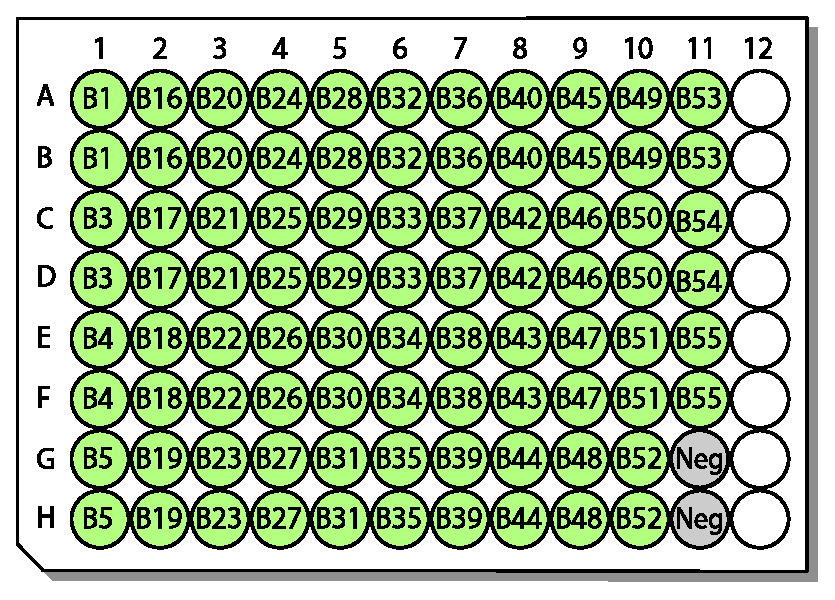
\includegraphics[width=8cm]{placaqpcr}
    \caption {Diseño de placa para PCR en tiempo real}
    \label {fig:placapcr}
\end{figure}

Cada reacción se llevó a cabo en un volumen de 10µl según la Tabla
\ref{mmix}. Las condiciones térmicas de la amplificación fueron las
siguientes: un ciclo inicial de 3 minutos a 95ºC (activación
enzimática), seguido por 39 ciclos de 5 segundos a 95ºC, 5 segundos a
58º para todos los partidores exceptuando los partidores para
IFN-\(\gamma\) que fue de 61,5º y 15 segundos a 72ºC (desnaturalización,
\emph{annealing} y extensión respectivamente).

\begin{table}[h!]
    \begin{center}
        \begin{threeparttable}
            \caption{Preparación de Master Mix para qPCR}\label{mmix}
                \begin{tabularx}{13cm}{X l}
                    \toprule
                                                            & \textbf{1 Reacción} \\
                    \midrule
                    Brilliant III Ultra-Fast SYBR Green MM  & 5\si{\micro\litro} \\
                    Partidores (F+R) 1,5\si{\micro\molar}   & 4\si{\micro\litro} \\
                    Muestra (1:4)                           & 1\si{\micro\litro} \\
                    \textbf{Total por reacción}             & 10m\si{\litro} \\
                    \bottomrule
                \end{tabularx}
                \begin{tablenotes}
                    \item Tabla de reactivos para 1 reacción de qPCR
                \end{tablenotes}
        \end{threeparttable}
    \end{center}
\end{table}

\subsection{Partidores}

\begin{table}[h!]
    \begin{center}
        \begin{threeparttable}
            \caption{Lista de Partidores}\label{tabla:partidores}
            \begin{tabularx}{15cm}{l l X r}
                \toprule
                \textbf{Molécula}   & \textbf{Partidor} & \textbf{Secuencia} & \textbf{Amplicón} \\
                \midrule
                EF-1$\alpha$        & Fw    & \texttt{TGG AGA CTG GCA CCC TGA AG}       & 127 pb    \\
                                    & Rev   & \texttt{CCA ACA TTG TCA CCA GGC ATG G}    &           \\
                IL-1$\beta$         & Fw    & \texttt{GTC ACA TTG CCA ACC TCA TCA TCG}  & 95 pb     \\
                                    & Rev   & \texttt{GTT GAG CAG GTC CTT GTC CTT GA}   &           \\
                TNF-$\alpha$        & Fw    & \texttt{GTG TGG GGT CCT CTT AAT AGC AGG}  & 88 pb     \\
                                    & Rev   & \texttt{CTG CAT CGT TGA CGG TCT TCC}      &           \\
                IFN-$\gamma$        & Fw    & \texttt{GCT GTT CAA CGG AAA ACC TGT TT}   & 51 pb     \\
                                    & Rev   & \texttt{TCA CTG TCC TCA AAC GTG}          &           \\
                iNOS                & Fw    & \texttt{TAT GCT CTG CCT GCC GTG TC}       & 158 pb    \\
                                    & Rev   & \texttt{ATC CTG CGA CCC ACT TCC TC}       &           \\
                IL-12               & Fw    & \texttt{TTT AAT CAG CTG TCG GGC CAA GTC}  & 123 pb    \\
                                    & Rev   & \texttt{GTG CAA GAT TCC TGG CTG TCA GTA}  &           \\
                \bottomrule                         
            \end{tabularx}
            \begin{tablenotes}[normal,flushleft,rm]
                \item Tabla de partidores usados para la amplificación de las moléculas en estudio, se indica el tamaño esperado en pares de bases del amplicón. \\ Fw = Forward, Rev= Reverse, pb = Pares de Bases
            \end{tablenotes}
        \end{threeparttable}
    \end{center}
\end{table}

\subsection{Estandarización de partidores}

Los partidores se estandarizaron con un mix de varios cDNA obtenidos en
este estudio usando distintas diluciones y gradientes de temperatura
dependiendo del partidor, seleccionando la mejor temperatura de
\emph{annealing} en base a su curva patrón y de fusión (Tabla
\ref{tabla:estandar}).

\begin{table}[h!]
    \begin{center}
        \begin{threeparttable}
            \caption{Programa Termociclador para estandarización de Partidores}\label{tabla:estandar}
            \begin{tabularx}{13cm}{l X l l}
                \toprule
                Etapa & Temperatura & Tiempo & Ciclos \\
                \midrule
                Denaturación Inicial & 95º & 03:00 min & 1 \\
                Denaturación & 95º & 00:10 seg & 39\\
                Annealing en Gradiente & 62º $\rightarrow$ 52* & 00:10 seg & 39 \\
                Extensión & 60º & 00:10 seg & 39 \\
                \bottomrule
            \end{tabularx}
            \begin{tablenotes}
                \item El gradiente varía dentro de esas temperaturas según los partidores
            \end{tablenotes}
        \end{threeparttable}
    \end{center}
\end{table}

\section{Extracción de Proteínas}

Se agregó una pequeña cantidad de tejido pulverizado a
500\si{\micro\litro} de Buffer de Lisis (Tabla \ref{tablabufferlisis}) y
se homogenizó con el equipo FastPrep24 con un programa de 4,5
movimientos por segundo durante 30 segundos usando como matriz 8 esferas
de óxido de zirconio, luego se dejaron las muestras en hielo durante 30
minutos para posteriormente centrifugar a máxima velocidad por 5 minutos
a 4ºC, se descartó el precipitado y el sobrenadante se almacenó a -80ºC
hasta su uso.

\begin{table}[h!]
    \begin{center}
        \begin{threeparttable}
            \caption{Composición Buffer de Lisis}\label{tablabufferlisis}
            \begin{tabularx}{10cm}{X l}
                \toprule
                Compuesto & Concentración \\
                \midrule
                Tris pH: 7,5 & 0,02M \\
                NaCl & 0,1M \\
                Tritón X-100 & 0,05\% \\
                PMSF & 5mM \\
                \emph{Cocktail} Inhibidor de Proteasas* & 0,2\% \\
                \bottomrule
            \end{tabularx}
            \begin{tablenotes}
                \item *\emph{Sigma Aldrich, P8340}
            \end{tablenotes}
        \end{threeparttable}
    \end{center}
\end{table}

\subsection{Cuantificación de Proteínas}
\label{cuantificacionbca}

Para cuantificar las proteínas totales extraídas se usó el método del
ácido bicinconínico (BCA, por sus siglas en inglés), el cual está basado
en la capacidad de este compuesto por formar un intenso complejo purpura
con el ion cuproso en un entorno básico, producido al reaccionar las
proteínas con cobre alcalino (método Biuret), y el BCA de cierta forma
va censando esta formación (Smith et~al., 1985). Se utilizará el Kit BCA
(Thermo Pierce), como curva de calibrado se usó albumina de suero bovino
(BSA, por sus siglas en inglés) en diferentes concentraciones (1,5; 1,0;
0,75; 0,5; 0,25; 0,125 y 0,0125 \si{\micro\gramo}/\si{\micro\litro}). En
una placa de cultivo de 96 pocillos se cargaron 25\si{\micro\litro} de
cada concentración de la curva de calibrado y 25\si{\micro\litro} de
cada extracto de proteínas en una dilución 1:50, todas las muestras
incluyendo la curva se cargaron en duplicado. Luego se agregaron 200
\si{\micro\litro} del reactivo BCA en una relación 50:1 (A:B) siguiendo
las instrucciones del fabricante, y se incubó la microplaca a 37ºC. Para
la lectura de la placa se usó un lector espectrofotométrico de
microplacas (VersaMax Microplate Reader, Molecular Devices) a una
longitud de onda de 562nm.

\section{ELISA Indirecto}

Para validar los anticuerpos en estudio y ademas, determinar
posteriormente la presencia de las moléculas en estudio se realizaron
ensayos de ELISA -del inglés \emph{Enzyme Linked Immunosorbent Assay}-
Indirecto.

\subsection{Activación de la placa}

La placa de 96 pocillos
PolySorp\textregistered (\emph{nunc\texttrademark}) se activó
\emph{overnight} en duplicado con 30ng de proteínas totales previamente
extraidas de branquias usando PBS 1X para diluir según sea necesario.
Todas las muestras se sembraron en duplicado, y como blanco se utilizó
PBS 1X. Luego se lavó 3 veces cada pocillo con 200\si{\micro\litro} de
PBS 1X-Tween20 0,05\% (PBST 0,05\%).

\subsubsection{Validación de anticuerpos}

Para la validación de anticuerpos en vez de sembrar una muestra de
proteinas totales, se sembró en concentración decreciente (8 diluciones
seriadas 1:2 desde 3ng/\si{\micro\litro}) el péptido (inmunógeno)
especifico para cada anticuerpo.

\subsection{Bloqueo de sitios inespecíficos}

Para bloquear los sitios inespecíficos donde no se unió el antígeno se
usó BSA diluida (200\si{\micro\litro} por pocillo)en PBS 1X al 1\% (PBSA
1\%) incubando la placa cubierta con parafilm por 2 horas a 37ºC con
agitación leve y luego lavando la placa 3 veces con 200\si{\micro\litro}
PBST 0,05\% usando un lavador de microplacas.

\subsection{Incubación primer anticuerpo}

El anticuerpo primario se usó a una concentración de 1:2000 o 1:1000
según corresponda (Tabla \ref{tabla:anticuerpos}) durante 1 hora a 37ºC
con agitación constante y luego se lavó nuevamente la placa 3 veces con
PBST 0,05\%

\subsection{Incubación segundo anticuerpo y revelado}

Se incubaron 100\si{\micro\litro} del anticuerpo secundario anti-conejo
o anti-ratón según corresponda en una dilución 1:5000 y 1:7000
respectivamente por 1 hora a 37ºC con agitación leve, posteriormente se
lavó la placa 3 veces con PBST 0,05\% y se incubó con TMB (3,3',
5,5;-tetrametilbencidina) (Invitrogen) por 30 minutos en oscuridad.
Luego se leyó la placa a 650nm y finalmente, deteniendo la reacción con
50\si{\micro\litro} de H\subindice{2}SO\subindice{4} 1N se leyó a 450nm
para aumentar la detección usando el software SoftMax 5.2 de Molecular
Probes.

\section{Cortes histológicos}

Desde las branquias previamente aisladas y fijadas en reactivo de Bouin,
se formaron bloques emparafinados, para posteriormente llevarlos a un
micrótomo, con la finalidad de poder obtener cortes a
5\si{\micro\meter}.

Para evaluar la integridad de los cortes histológicos previamente
preparados se procedió a realizar una tinción hematoxilina-eosina,
tinción que nos permite distinguir nucleos y otros componentes celulares
(Sharpey-Schäfer y Carleton, 1938).

\subsection{Tinción Hematoxilina-eosina}

Los cortes se desparafinaron con NeoClear\textregistered (Merck) como
sustituto de xileno, luego, para hidratarlos se pasaron los portaobjetos
por una batería de alcohol decreciente (100º-96º-70º) y finalmente se
sumergieron en agua.

Luego se tiñeron con Hematoxilina de Mayer (Merck) por un minuto y se
lavaron en agua por 5 minutos y se pasaron por agua desstilada.

Los cortes se deshidrataron usando una batería creciente de alcoholes
(70º-96º) y luego se tiñeron con Eosina durante 1 minuto. Para terminar
la deshidratación se pasaron 3 veces por alcohol 100º y finalmente la
muestra se aclaró 3 veces con NeoClear\textregistered.

Finalmente, el montaje se realizó usando Entellán (Merck) y se
obtuvieron microfotografías usando el Microscopio Leica DM4000B (Leica
Microsystems).

\section{Inmunofluorescencia}\label{sec:ifat}

Para localizar las moleculas en estudio se realizó una prueba de inmuno
fluorescencia con anticuerpos (IFAT).

\subsection{Desparafinización e Hidratación}

Los cortes previamente emparafinados se les quitó la parafina
incubandolos 2 veces durante 5 minutos en NeoClear\textregistered como
sustituto de xileno, para luego hidratar la muestra pasando por una
batería de alcoholes de 100\%, 96\% y 50\% durante dos minutos cada uno,
para finalizar lavando con Agua \emph{Milli-Q} (MQ) durante 5 minutos.

\subsection{Bloqueo}

Los cortes fijados en el portaobjetos fueron delimitados en cuadrantes
con un lapiz con tinta hidrofóbica (PAP PEN, Em sciences) para evitar la
posible perdida de material en las sucesivas incubaciones. Para preparar
la muestra para el bloqueo se incubó con PBS 1X y luego con PBST 0,05\%
durante 5 minutos cada uno. Para bloquear los sitios de union
inespecíficos en los tejidos se bloqueó durante 30 minutos con una
solución compuesta de PBSA 5\% con 0,3\% de Triton-X100 como potenciador
para la penetración del PBSA en el tejido. Luego de esto los cortes se
lavaron por 5 minutos con PBS 1X y PBST 0,05\% cada uno.

\subsection{Incubación de anticuerpo primario}

El anticuerpo primario se diluyó en PBSA 1\% según corresponda (Tabla
\ref{tabla:anticuerpos}) y se agregaron aproximadamente
50\si{\micro\litro} por cada tejido. La incubación fue en oscuridad
durante 1 hora a temperatura ambiente. Posteriormente se lavó con PBS 1X
y PBST 0,05\% con agitación durante 5 minutos cada uno.

\subsection{Incubación anticuerpo secundario y tinción de DNA (Núcleos)}

El anticuerpo secundario conjugado con el fluoroforo Alexa 568 y 635
anti ratón y conejo respectivamente se diluyeron según corresponda en
PBSA 1\% (Tabla \ref{tabla:anticuerpos-comerciales}) y se incubaron
durante 1 hora las muestras con esta solución a temperatura ambiente y
oscuridad. Posteriormente se lavó 1 vez con PBS 1X y 2 veces con PBST
0,05\% durante 10 minutos. Para teñir el DNA se utilizó SYTO9 (Life
Technologies) diluído en PBS 1X en una relación 1:1000 y se incubó por 5
segundos para finalmente lavar 3 veces con PBST 0,05\%

\subsection{Montaje}

El montaje fue realizado usando el medio de Montaje VECTASHIELD para
Inmunofluorescencia (VectorLabs) agregando 25\si{\micro\litro} sobre el
portaobjetos y luego superponiendo un cubre portaobjetos rectangular,
con mucho cuidado se presionó para distribuir el medio en todas las
muestras y se selló con esmalte para uñas. Finalmente los cortes se
almacenaron a 4º en oscuridad hasta su uso en el microscopio confocal.

\section{Microscopía Confocal}

La toma de imágenes se realizó con el Microscopio Confocal TCS SP5 II de
Leica Microsystems, cortesía del Nucleo Biotecnológico de Curauma (NBC).

\section{Analisis Estadístico}

Todos los análisis estadísticos fueron realizados en el software Prism
6.0 de GraphPad, la significancia fue obtenida usando la prueba pareada
de t de student con un 95\% de confianza (\(\alpha\) = 0.05).

\subsection{Coeficiente de correlación de Pearson (R)}

Para poder interpretar mejor los resultados, y ver como se relacionan
estos entre sí incluso entre técnicas diferentes, se realizaron duplas
entre cada uno de estos datos. Con estas duplas finalmente se calculó el
coeficiente de correlación de Pearson (R), el cual puede ser calculado
con la siguiente ecuación

\begin{equation}
    R = \frac{   \sum{X Y} - \frac{ (\sum{X})(\sum{Y})}{n}              }
            { \sqrt{ \left( \sum{X^2} -\frac{ (\sum{X})^2}{n} \right)
            \left( \sum{Y^2} -\frac{ (\sum{Y})^2}{n} \right) } }
\end{equation}

\chapter{Resultados}

\vfill
Los resultados se expresarán en base a su relación con los objetivos
específicos. \vfill
\clearpage

\epigraph{\textbf{Objetivo 1}: ``Implementar un sistema de alimentación que permita realizar la administración oral de zimosán y sus respectivos controles a O.mykiss.''}

\section{Bioensayo}

Se implementó el sistema de alimentación para las truchas arcoiris en el
CIAC, donde se contó con 2 modulos de 3 estanques cada uno, dos de los
cuales fueron destinados a la alimentación con la dieta suplementada con
zimosán (estanques 2 y 5) y otros dos a la dieta control (estanques 1 y
4) (Fig. \ref{fig:ciac}).

\begin{figure}[h!]
    \centering
    \fbox{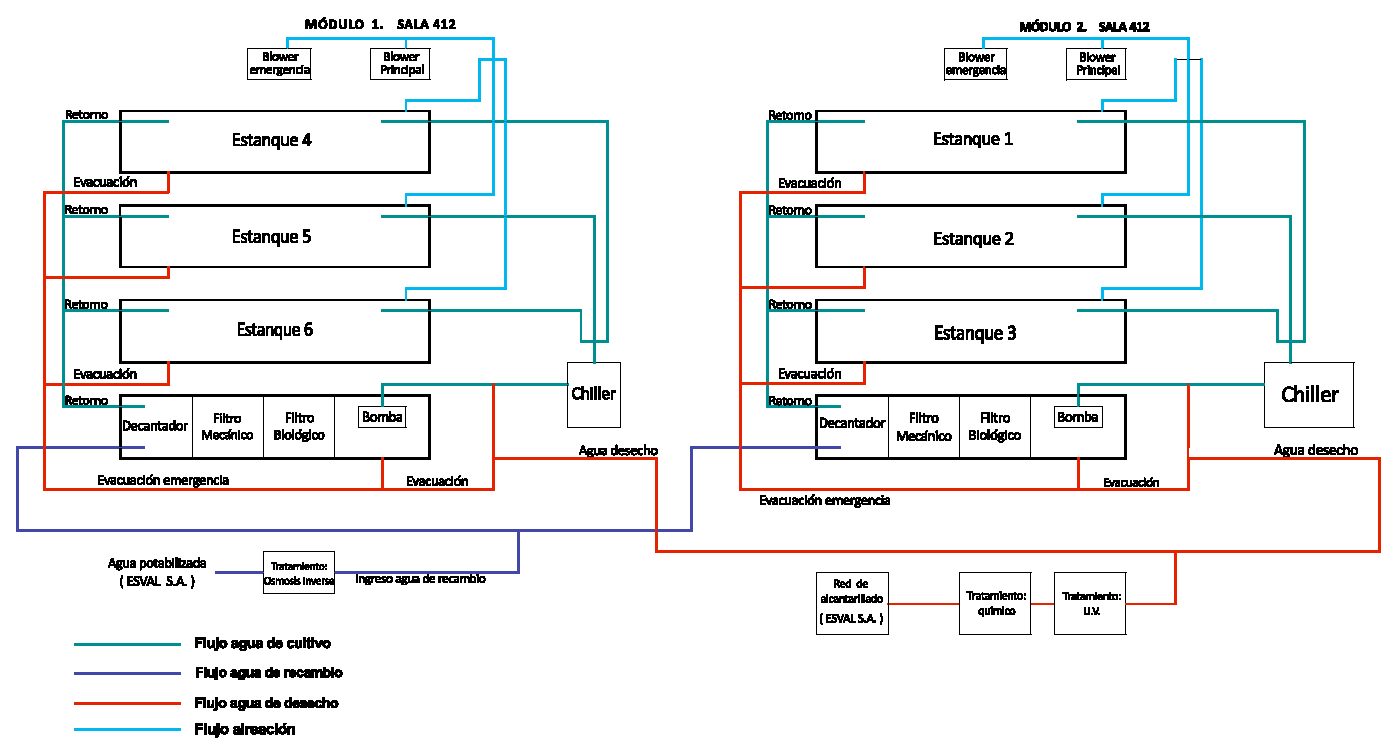
\includegraphics[width=13cm]{ciac}}
    \caption {Diagrama de flujo Centro de Investigaciones en Acuicultura Curauma}
    \label {fig:ciac}
\end{figure}

\begin{figure}[h!]
    \centering
    \fbox{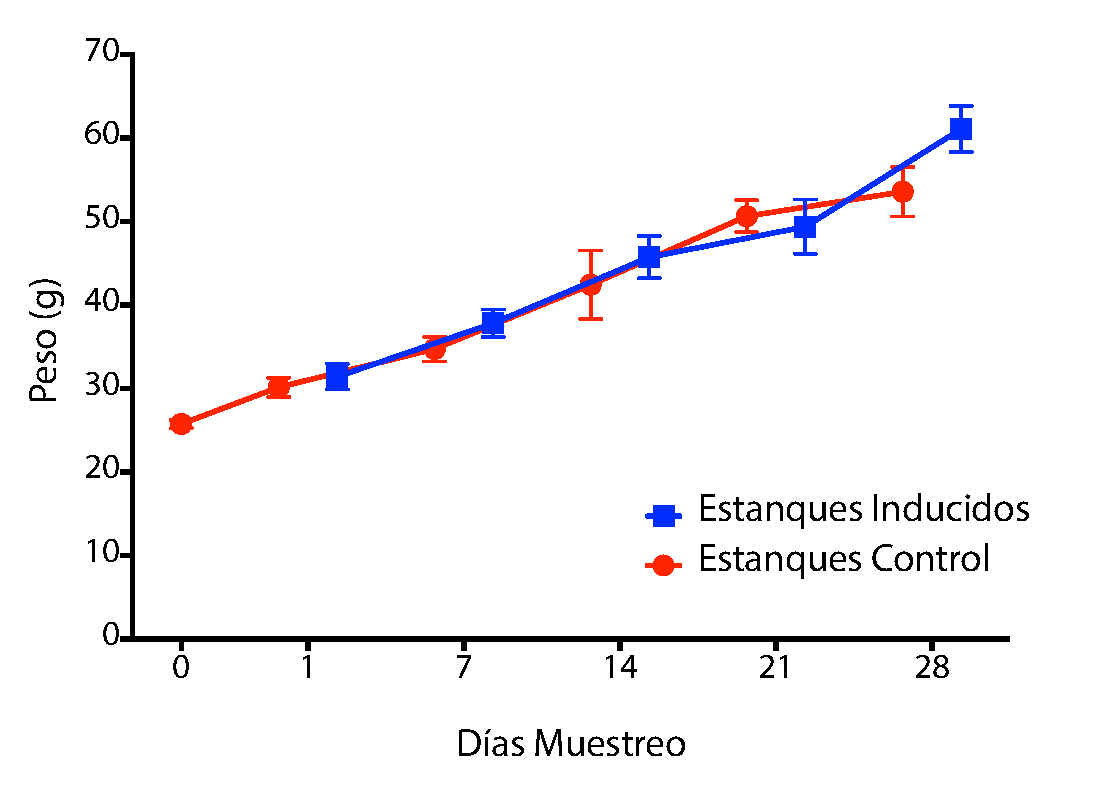
\includegraphics[width=7cm]{peso}}
    \caption {Crecimiento promedio de truchas en estudio}
    \label {fig:pesos}
\end{figure}

Al momento de sacrificar las truchas por sobre-sedación se procedió a
pesarlas, comparando la dieta control y la con \(\beta\)-glucanos para
evaluar si la alimentación generaba algun cambio de peso comparando con
el control (Figura \ref{fig:pesos}). Tampoco hubo otra causa de muerte
que no fuera el sacrificio en el bioensayo.

\clearpage

\epigraph{\textbf{Objetivo 2}: ``Evaluar la expresión de moléculas efectoras y reguladoras de respuesta inmune en tejido branquial de \emph{O.mykiss} tratados con Zymosán A liberado en dieta.''}

\section{Extracción y Cuantificación de RNA}

Se obtuvieron las siguientes cuantificaciones de RNA

\begin{table}[h!]
    \begin{center}
        \begin{threeparttable}
            \caption{Concentraciones de RNA total extraído}\label{tablaRNA}
            \begin{tabular}{l r l r l r l r l r}
                \toprule
                \textbf{ID}   & \textbf{ng/µL} & \textbf{ID} & \textbf{ng/µL} & \textbf{ID} & \textbf{ng/µL} & \textbf{ID} & \textbf{ng/µL} & \textbf{ID} & \textbf{ng/µL}\\
                \midrule
                B1    & 151,40 & B21 & 257,00 & B31 & 242,10 & B41 & 40,20 & B51 & 264,10 \\
                B2 & 63,30 & B22 & 341,50 & B32 & 250,40 & B42 & 121,90 & B52 & 183,00 \\
                B3 & 208,40 & B23 & 145,10 & B33 & 264,10 & B43 & 105,20 & B53 & 393,40 \\
                B4 & 178,30 & B24 & 121,30 & B34 & 295,10 & B44 & 237,30 & B54 & 292,80 \\
                B5 & 248,40 & B25 & 151,70 & B35 & 572,70 & B45 & 116,40 & B55 & 322,60 \\
                B16 & 165,10 & B26 & 326,30 & B36 & 115,60 & B46 & 415,60 & \\
                B17 & 249,90 & B27 & 149,30 & B37 & 183,20 & B47 & 220,80 & \\
                B18 & 138,40 & B28 & 263,90 & B38 & 171,60 & B48 & 271,40 & \\
                B19 & 169,60 & B29 & 357,30 & B39 & 194,50 & B49 & 173,80 & \\
                B20 & 690,70 & B30 & 341,80 & B40 & 192,40 & B50 & 315,40 & \\
                \bottomrule
            \end{tabular}
        \end{threeparttable}
    \end{center}
\end{table}

Luego teniendo esas concentraciones se procedió a la síntesis del cDNA
usando 1µg de RNA para poder realizar los ensayos de PCR en tiempo real.

\section{Estandarización de Partidores}

Usando un mix de varios cDNA al azar (controles e inducidos) se
estandarizaron los distintos partidores usados en el ensayo, usando
diluciones en agua DEPC 1:1 1:2 1:4 1:8 de este mix en cada placa, por
cada partidor, luego el software CFX Manager (BioRad) entregará las
informaciones necesarias para determinar el uso o no de un partidor,
para los resultados de este tema se muestran las temperaturas de
annealing para las cuales los partidores dieron solo un producto, como
se demuestra en las curvas de disociación o de fusión, y hayan tenido
una eficacia cercana al 100\%.

\subsection{EF-1$\alpha$}

Se cargó 1µL de cada dilución del mix de cDNA y usando el programa del
termociclador correspondiente (Tabla \ref{tabla:estandar}), teniendo
como mejor curva estándar, eficiencia y curva de fusión a los 58ºC
(Figura \ref{fig:ef1a}).

\begin{figure}[h]
    \centering
        \subcaptionbox{Amplificación\label{fig:ef1a:ampl}}
        {\includegraphics[width=0.32\textwidth]{standarization/ef1a/ampl}}
        \subcaptionbox{Estandarización\label{fig:ef1a:stand}}
        {\includegraphics[width=0.32\textwidth]{standarization/ef1a/stand}}
        \subcaptionbox{Disociación\label{fig:ef1a:melting}}
        {\includegraphics[width=0.32\textwidth]{standarization/ef1a/melting}}
        \caption{Curvas de estandarización del partidor para EF-1$\alpha$}
    \label {fig:ef1a}
\end{figure}

\subsection{IL-12}

Se cargó 1µL de cada dilución del mix de cDNA y usando el programa del
termociclador correspondiente (Tabla \ref{tabla:estandar}), teniendo
como mejor curva estándar, eficiencia y curva de fusión a los 58ºC.
(Figura \ref{fig:il12})

\begin{figure}[h!]
    \centering
        \subcaptionbox{Amplificación\label{fig:il12:ampl}}
        {\includegraphics[width=0.32\textwidth]{standarization/il12/ampl}}
        \subcaptionbox{Estandarización\label{fig:il12:stand}}
        {\includegraphics[width=0.32\textwidth]{standarization/il12/stand}}
        \subcaptionbox{Disociación\label{fig:il12:melting}}
        {\includegraphics[width=0.32\textwidth]{standarization/il12/melting}}
        \caption{Curvas de estandarización del partidor para IL-12}
        \label {fig:il12}
\end{figure}

\subsection{TNF-$\alpha$}

Se cargó 1µL de cada dilución del mix de cDNA y usando el programa del
termociclador correspondiente (Tabla \ref{tabla:estandar}), teniendo
como mejor curva estándar, eficiencia y curva de fusión a los 58ºC
(Figura \ref{fig:tnfa}).

\begin{figure}[h!]
\centering
   \subcaptionbox{Amplificación\label{fig:tnfa:ampl}}
        {\includegraphics[width=0.32\textwidth]{standarization/tnfa/ampl}}
        \subcaptionbox{Estandarización\label{fig:tnfa:stand}}
        {\includegraphics[width=0.32\textwidth]{standarization/tnfa/stand}}
        \subcaptionbox{Disociación\label{fig:tnfa:melting}}
        {\includegraphics[width=0.32\textwidth]{standarization/tnfa/melting}}
        \caption{Curvas de estandarización del partidor para TNF-$\alpha$}
    \label {fig:tnfa}
\end{figure}

\subsection{IFN-$\gamma$}

Se cargó 1µL de cada dilución del mix de cDNA y usando el programa del
termociclador correspondiente (Tabla \ref{tabla:estandar}), teniendo
como mejor curva estándar, eficiencia y curva de fusión a los 61.5ºC
(Figura \ref{fig:ifng}).

\begin{figure}[h!]
\centering
        \subcaptionbox{Amplificación\label{fig:ifng:ampl}}
        {\includegraphics[width=0.32\textwidth]{standarization/ifng/ampl}}
        \subcaptionbox{Estandarización\label{fig:ifng:stand}}
        {\includegraphics[width=0.32\textwidth]{standarization/ifng/stand}}
        \subcaptionbox{Disociación\label{fig:ifng:melting}}
        {\includegraphics[width=0.32\textwidth]{standarization/ifng/melting}}
         \caption{Curvas de estandarización del partidor para IFN-$\gamma$}
         \label {fig:ifng}
    \end{figure}

\subsection{IL-1$\beta$}

Se cargó 1µL de cada dilución del mix de cDNA y usando el programa del
termociclador correspondiente (Tabla \ref{tabla:estandar}), teniendo
como mejor curva estándar, eficiencia y curva de fusión a los 58ºC
(Figura \ref{fig:il1b}).

\begin{figure}[h!]
\centering
   \subcaptionbox{Amplificación\label{fig:il1b:ampl}}
        {\includegraphics[width=0.32\textwidth]{standarization/il1b/ampl}}
        \subcaptionbox{Estandarización\label{fig:il1b:stand}}
        {\includegraphics[width=0.32\textwidth]{standarization/il1b/stand}}
        \subcaptionbox{Disociación\label{fig:il1b:melting}}
        {\includegraphics[width=0.32\textwidth]{standarization/il1b/melting}}
        \caption{Curvas de estandarización del partidor para IL-1$\beta$}
    \label {fig:il1b}
\end{figure}

\subsection{iNOS}

Se cargó 1µL de cada dilución del mix de cDNA y usando el programa del
termociclador correspondiente (Tabla \ref{tabla:estandar}), teniendo
como mejor curva estándar, eficiencia y curva de fusión a los 58ºC
(Figura \ref{fig:inos}).

\begin{figure}[h!]
\centering
   \subcaptionbox{Amplificación\label{fig:inos:ampl}}
        {\includegraphics[width=0.32\textwidth]{standarization/inos/ampl}}
        \subcaptionbox{Estandarización\label{fig:inos:stand}}
        {\includegraphics[width=0.32\textwidth]{standarization/inos/stand}}
        \subcaptionbox{Disociación\label{fig:inos:melting}}
        {\includegraphics[width=0.32\textwidth]{standarization/inos/melting}}
        \caption{Curvas de estandarización del partidor para iNOS}
    \label {fig:inos}
\end{figure}

Al ya tener las temperaturas de \emph{annealing} definidas para cada
partidor se procedió a realizar el PCR en tiempo real para todas las
muestras en estudio y posteriormente evaluar la expresión n relativa al
gen de referencia.

\section{PCR en tiempo real}

Para evaluar la cuantificación relativa de cada gen en estudio frente al
gen de referencia, en este caso el factor de elongación 1 alfa
(EF-1\(\alpha\)), se utilizo la metodología llamada \(\Delta\Delta C_T\)
(M. W. Pfaffl, 2001), la cual consiste en lo siguiente: el valor
\(\Delta C_T\) se determina restando la media de los valores \(C_T\)
obtenidos para el gen de referencia de la media de los valores \(C_T\)
del gen problema.

Por otra parte, en todas las muestras el valor de \(C_T\) obtenido para
el gen EF-1\(\alpha\) fue similar, lo que indicaba que las
amplificaciones se desarrollaron de forma correcta y que en todas las
reacciones se partió de cantidades similares de cDNA (Figura
\ref{qef1a}).

El cálculo del valor \(\Delta\Delta C_T\) implica restar a cada
\(\Delta C_T\) el valor del \(\Delta C_T\) de un calibrador, que es una
muestra utilizada como base para los resultados relativos. Al ser una
resta de un valor arbitrario, la desviación del \(\Delta\Delta C_T\) es
la misma que la del \(\Delta C_T\) . Una vez obtenidos estos valores, la
cantidad de un gen problema, normalizado a una referencia endógena y
relativa a un calibrador, viene dada por la fórmula:

\begin{displaymath}
\scalebox{1.5}{
$2^{-\Delta\Delta C_T}$
}
\end{displaymath}

\begin{figure}[h!]
    \centering
    \begin{subfigure}{0.32\textwidth}
        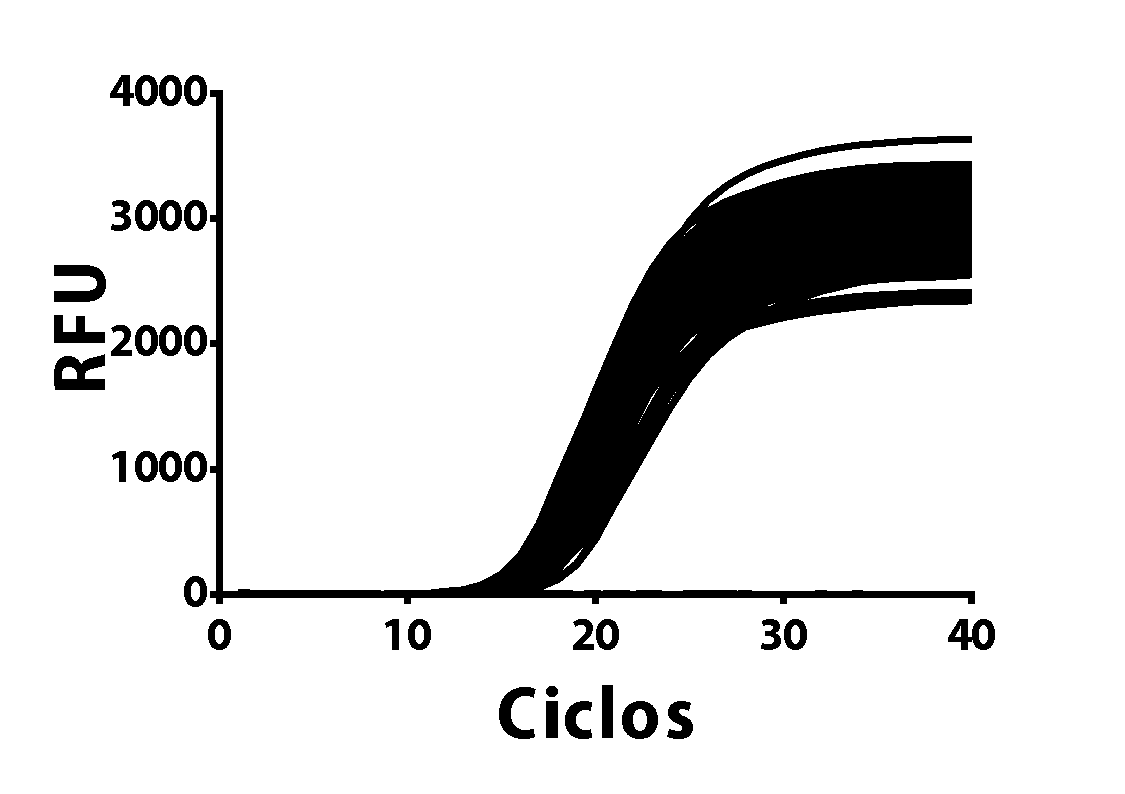
\includegraphics[width=1\textwidth]{qef1a}
        \caption{Curva de amplificación}
        \end{subfigure}
    \begin{subfigure}{0.32\textwidth}
        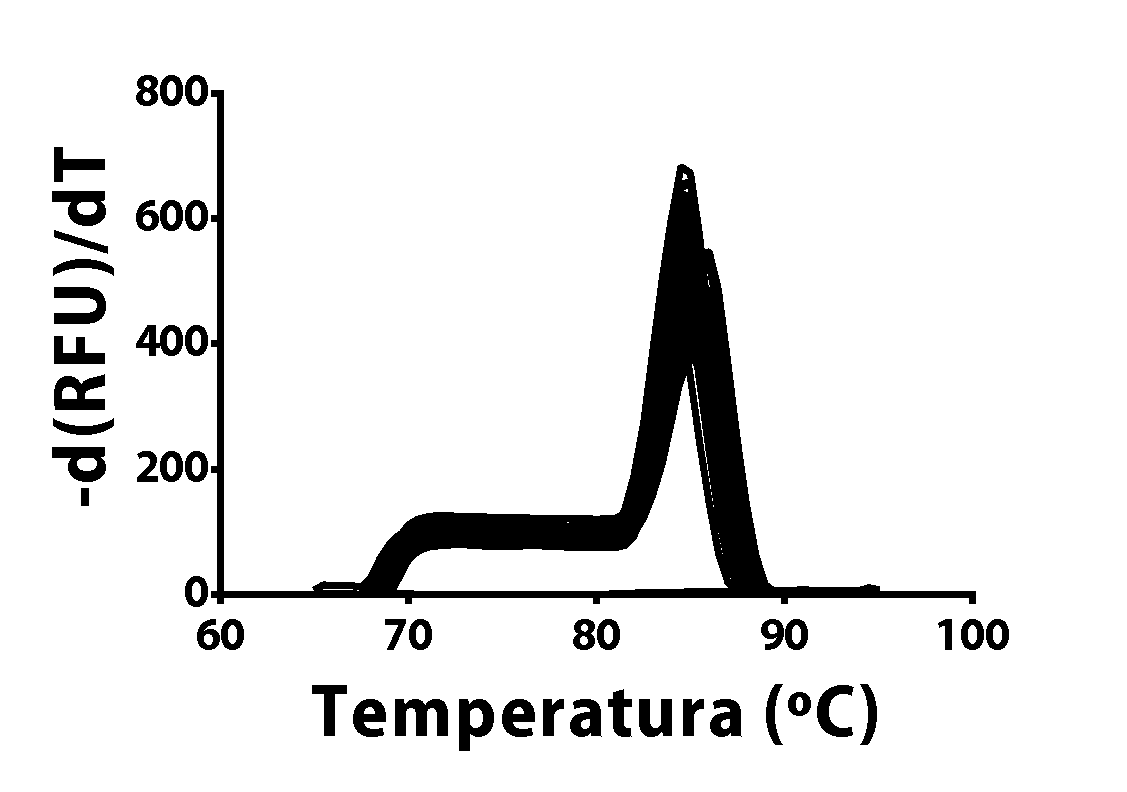
\includegraphics[width=01\textwidth]{qef1am}
        \caption{Curva de disociación}
    \end{subfigure}
    \caption{Reacción de PCR en Tiempo real para el gen de referencia EF-1a}
    \label{qef1a}
\end{figure}

\begin{figure}[h!]
    \begin{subfigure}{0.5\textwidth}
        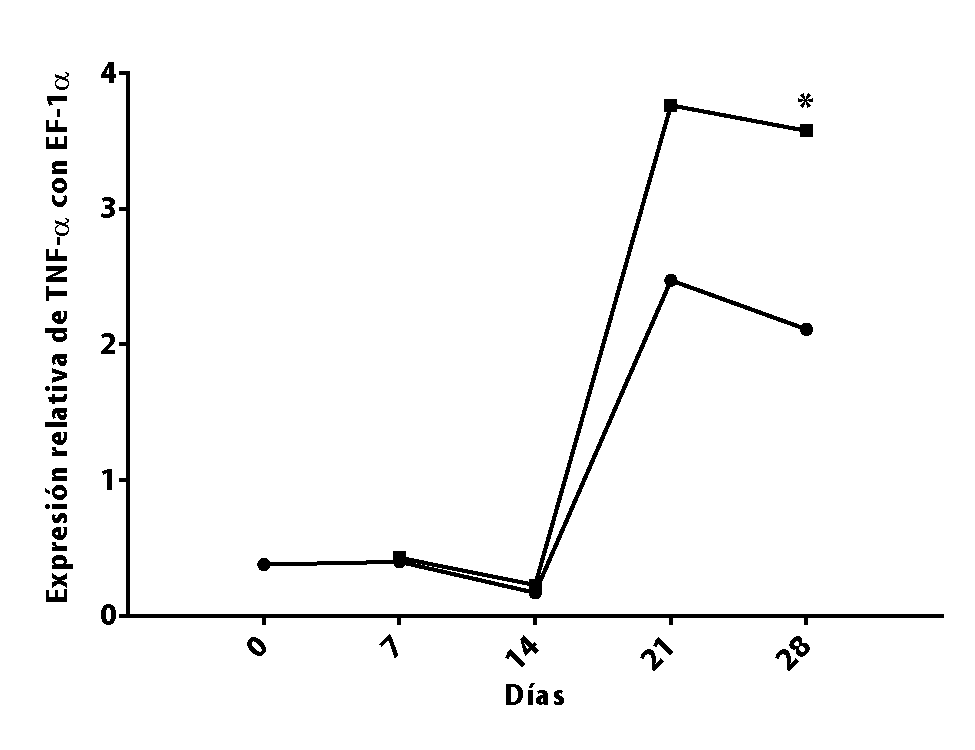
\includegraphics[width=0.9\textwidth]{eps/qPCR/qtnfa}
        \caption{TNF-$\alpha$}
        \label{fig:qpcr:tnfa}
        \end{subfigure}
    \begin{subfigure}{0.5\textwidth}
        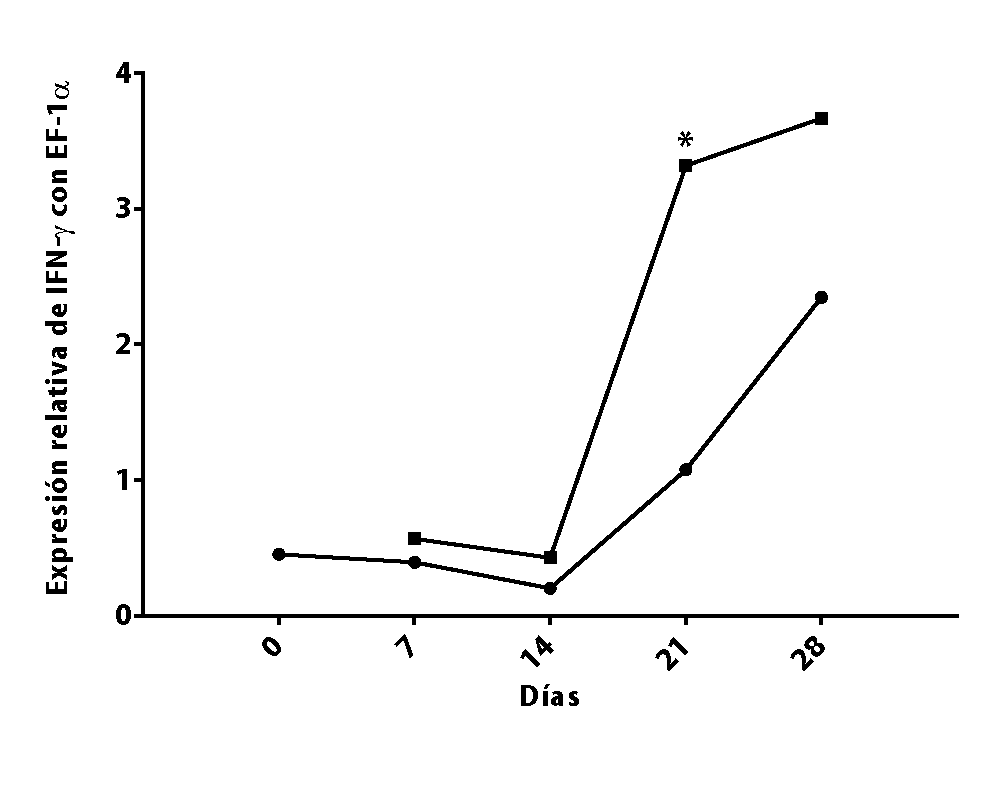
\includegraphics[width=0.9\textwidth]{eps/qPCR/qifng}
        \caption{IFN-$\gamma$}
        \label{fig:qpcr:ifng}
    \end{subfigure}
    \begin{subfigure}{0.5\textwidth}
        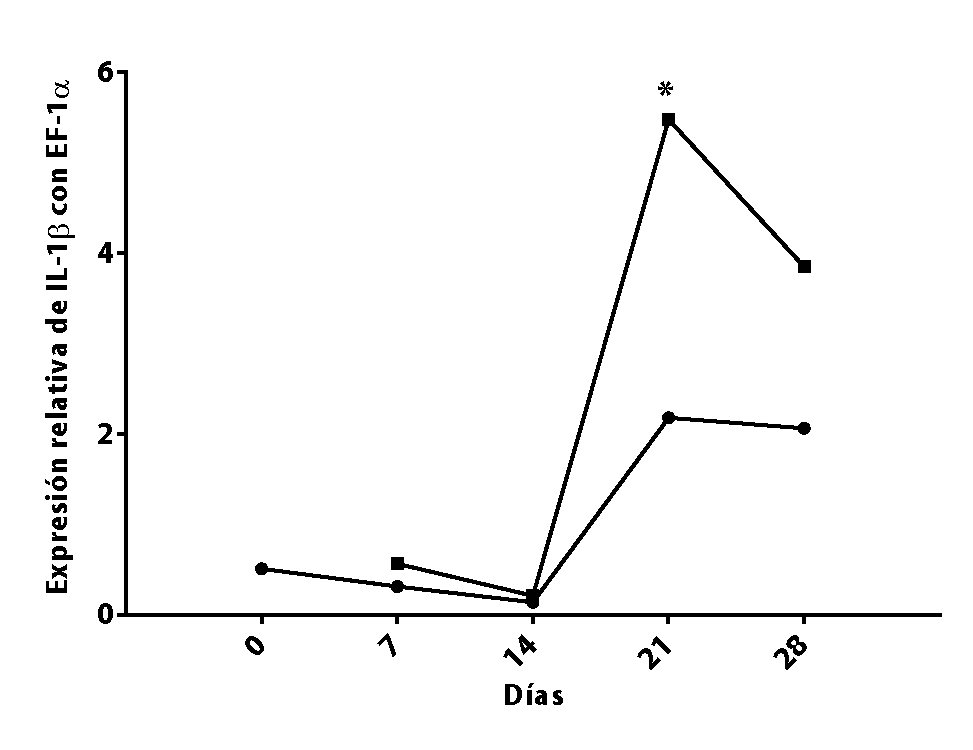
\includegraphics[width=0.9\textwidth]{eps/qPCR/qil1b}
        \caption{IL-1$\beta$}
        \label{fig:qpcr:il1b}
    \end{subfigure}
    \begin{subfigure}{0.5\textwidth}
        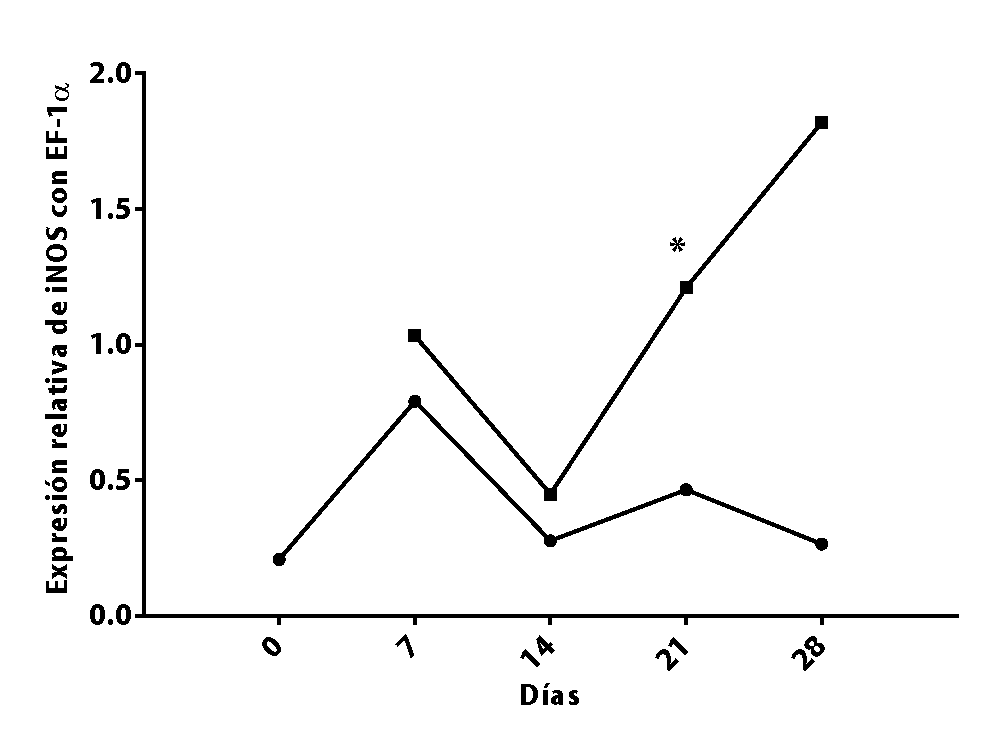
\includegraphics[width=0.9\textwidth]{eps/qPCR/qinos}
        \caption{iNOS}
        \label{fig:qpcr:inos}
    \end{subfigure}
    \begin{subfigure}{0.5\textwidth}
        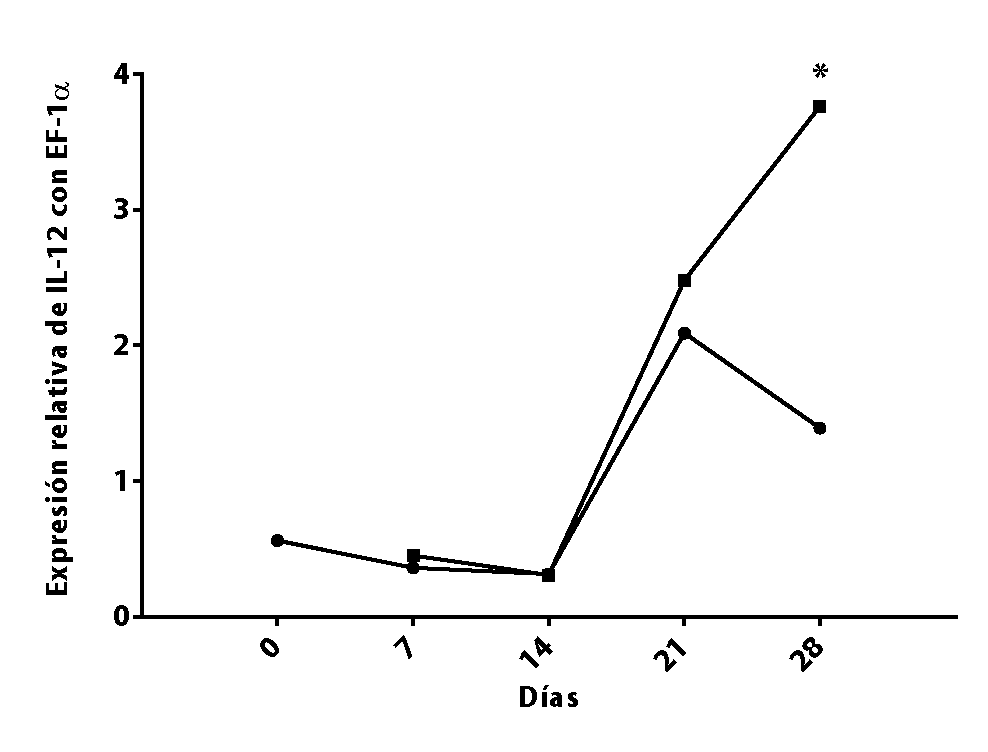
\includegraphics[width=0.9\textwidth]{eps/qPCR/qil12}
        \caption{IL-12}
        \label{fig:qpcr:il12}
    \end{subfigure}
    \begin{subfigure}{0.5\textwidth}
        \includegraphics[width=0.9\textwidth]{eps/qPCR/leyenda}
    \end{subfigure}
    \caption{Expresión relativa de los genes en estudio frente a EF-1$\alpha$}
    \label{fig:qpcr}
\end{figure}

\subsection{TNF-$\alpha$}

Para el gen del factor de necrosis tumoral alfa
(\ref{fig:qpcr}\subref{fig:qpcr:tnfa}) la expresión de transcrito se
mantuvo constante en condiciones controles y tratadas hasta el día 14,
donde aumentó súbitamente la cantidad relativa de mensajero en ambas
circunstancias hasta llegar a su máximo \emph{peak} el día 21,
finalmente baja un poco su expresión el día 28, día en el cual hubo una
diferencia significativa con su control(\(p \leq 0,05\)).

\subsection{IFN-$\gamma$}

La expresión relativa del transcrito de Interferón gamma
(\ref{fig:qpcr}\subref{fig:qpcr:ifng}) frente al gen de referencia en
condiciones control y tratadas se mantuvieron en bajas cantidades hasta
el día 14, 7 días después hubo un peak significativo comparado con su
control (\(p \leq 0,05\)), cabe destacar que los días 21 y 28 en
situaciones control hubo un aumento de transcrito para este gen, aunque
no significativo con sus pares tratados.

\subsection{IL-1$\beta$}

Al igual que los dos genes anteriores, la expresión de interleuquina 1
beta (\ref{fig:qpcr}\subref{fig:qpcr:il1b}) se mantuvo baja los primeros
14 días con respecto al control inicial, para luego el día 21 aumentar
súbita y significativamente (\(p \leq 0,05\)) en condiciones tratadas
frente a su control del día, finalmente el día 28 baja la expresión del
transcrito mientras que el control se mantiene estable.

\subsection{iNOS}

El gen de iNOS (\ref{fig:qpcr}\subref{fig:qpcr:inos}) el día 7 se empezó
a transcribir demostrando un aumento en ambas condiciones frente al
control inicial, para luego bajar su expresión casi al nivel del día 0,
luego, en condiciones tratadas, este gen experimenta una gran expresión
frente al gen de referencia (\(p \leq 0,05\)), siendo significativa el
día 21, y subiendo hasta el día 28. En los peces controles, desde el día
14 al 28 se mantuvo prácticamente constante.

\subsection{IL-12}

El comportamiento de Interleuquina 12
(\ref{fig:qpcr}\subref{fig:qpcr:inos}) tiene cierta tendencia comparado
con la expresión del gen para IL-1\(\beta\), ya que también se gatilla
su expresión el día 14, aunque para el caso de esta citoquina, el día 28
es su mayor \emph{peak} siendo significativo este con respecto a su
control (\(p \leq 0,05\)).

\clearpage

\epigraph{\textbf{Objetivo 3}: ``Detectar la disponibilidad de proteínas efectoras y reguladoras de respuesta inmune en tejido branquial de O.mykiss tratados con Zymosán A liberado en dieta.''}

\section{Extracción y Cuantificación de Proteínas}

Con los datos obtenidos por el lector espectrofotométrico de
microplacas, usando las concentraciones sembradas de BSA, se construyó
la curva de calibrado para la cuantificación de proteínas. Obteniendo el
siguiente gráfico y ecuación de la recta:

\begin{figure}[h!]
\centering
    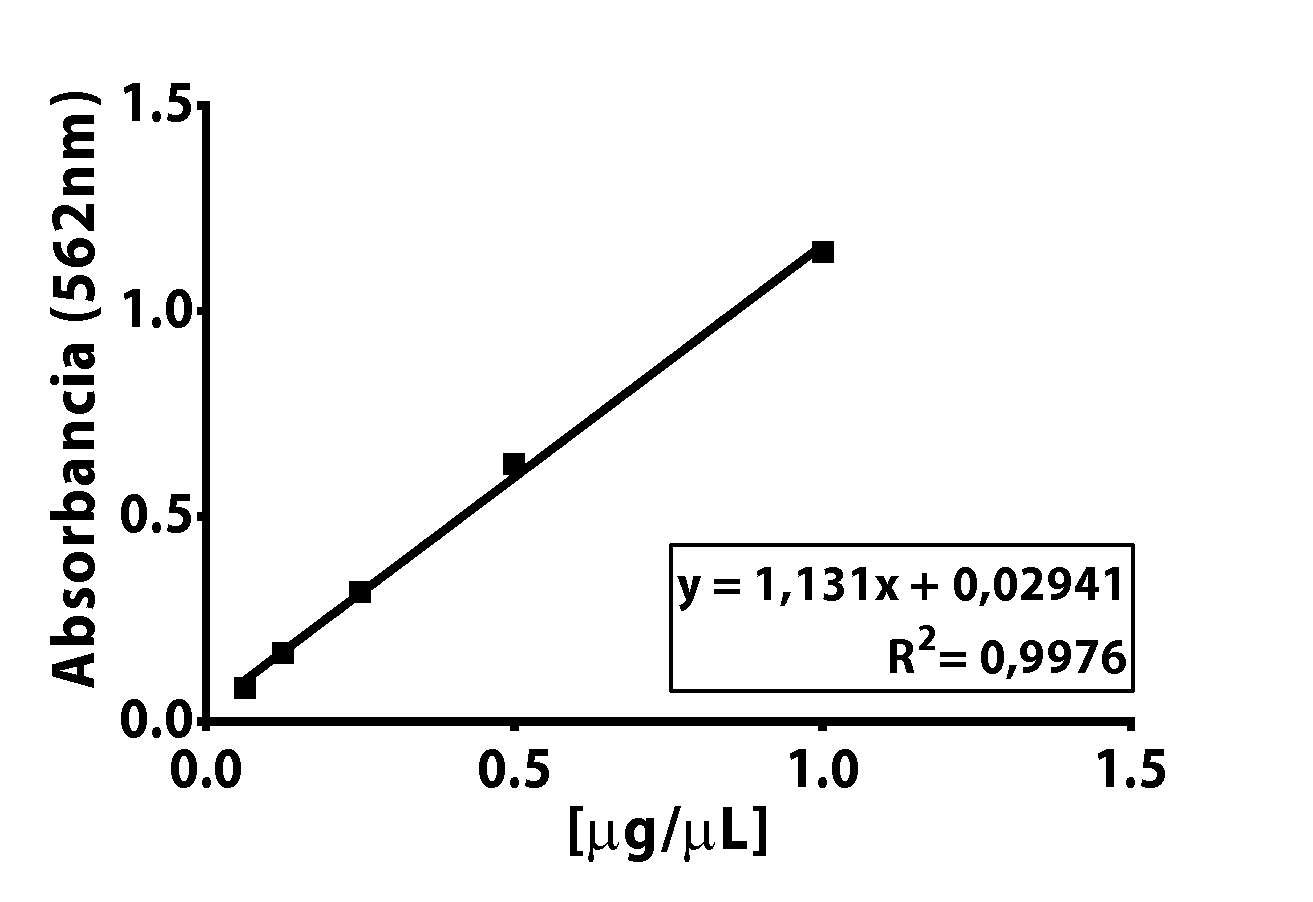
\includegraphics[width=0.4\textwidth]{BCA}
    \caption{Curva de calibrado BCA}
    \label{curvabca}
\end{figure}

\begin{displaymath}
y=1,131x+0,02941
\label{eq:BCA}
\end{displaymath}

Interpolando en la recta de calibrado (Figura \ref{curvabca}) las
absorbancias obtenidas en el metodo BCA, se obtuvieron las siguientes
concentraciones de proteínas.

\begin{table}[h]
\begin{center}
    \begin{threeparttable}
      \caption{Concentraciones de Proteínas totales extraidas}\label{tablaPROTEINAS}
      \begin{tabular}{l r l r l r l r l r}
    \toprule
    \textbf{ID} & \textbf{µg/µL} & \textbf{ID} & \textbf{µL/µL} & \textbf{ID} & \textbf{µL/µL} & \textbf{ID} & \textbf{µL/µL} & \textbf{ID} & \textbf{µL/µL}\\
    \midrule
    B1 & 4,14 & B21 & 3,79 & B31 & 4,10 & B41 & 3,35 & B51 & 2,70 \\
    B2 & 3,83 & B22 & 2,51 & B32 & 3,02 & B42 & 7,42 & B52 & 5,65 \\
    B3 & 3,84 & B23 & 3,20 & B33 & 9,62 & B43 & 5,20 & B53 & 4,31 \\
    B4 & 3,64 & B24 & 5,41 & B34 & 5,02 & B44 & 4,15 & B54 & 5,54 \\
    B5 & 3,66 & B25 & 6,43 & B35 & 5,88 & B45 & 6,62 & B55 & 3,18 \\
    B16 & 3,22 & B26 & 6,01 & B36 & 7,69 & B46 & 2,77 & \\
    B17 & 3,67 & B27 & 3,05 & B37 & 6,03 & B47 & 6,65 & \\
    B18 & 2,67 & B28 & 5,11 & B38 & 3,35 & B48 & 5,32 & \\
    B19 & 4,67 & B29 & 5,50 & B39 & 12,32 & B49 & 4,05 & \\
    B20 & 2,94 & B30 & 3,22 & B40 & 2,45 & B50 & 3,82 & \\
\bottomrule
\end{tabular}
\end{threeparttable}
\end{center}
\end{table}

\section{Validación de anticuerpos}

Se realizó la validación cualitativa de los anticuerpos policlonales
mono-específicos sintetizados por el grupo (Tabla
\ref{tabla:anticuerpos}) usando como antígeno específico el péptido
sintético (inmunógeno) con el cual fue inmunizado el huésped (conejo o
ratón) al momento de producir el anticuerpo.

\begin{figure}[h]
    \begin{subfigure}{0.5\textwidth}
        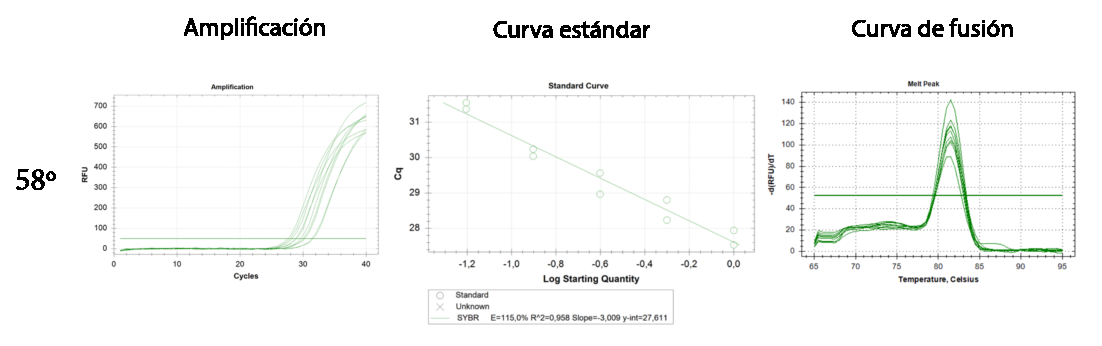
\includegraphics[width=0.9\textwidth]{peptidos/tnfa}
        \caption{TNF-$\alpha$}
        \label{fig:pep:tnfa}
        \end{subfigure}
    \begin{subfigure}{0.5\textwidth}
        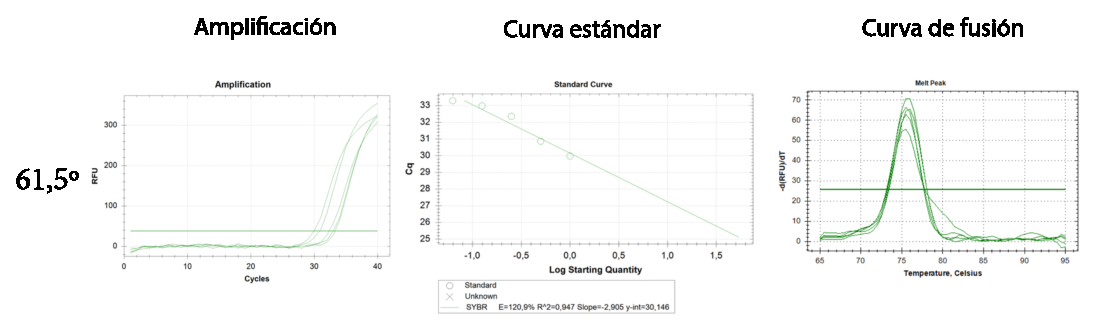
\includegraphics[width=0.9\textwidth]{peptidos/ifng}
        \caption{IFN-$\gamma$}
        \label{fig:pep:ifng}
    \end{subfigure}
      \begin{subfigure}{0.5\textwidth}
        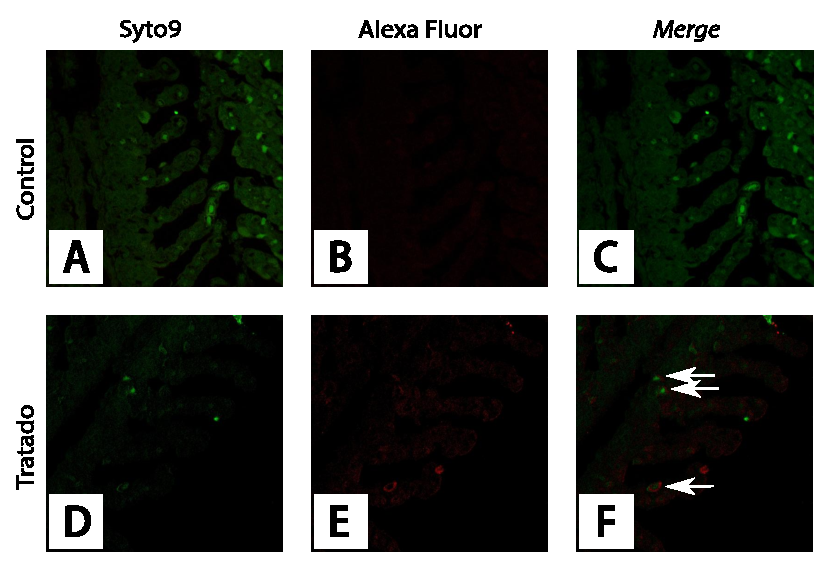
\includegraphics[width=0.9\textwidth]{peptidos/il1b}
        \caption{IL-1$\beta$}
        \label{fig:pep:il1b}
    \end{subfigure}
     \begin{subfigure}{0.5\textwidth}
        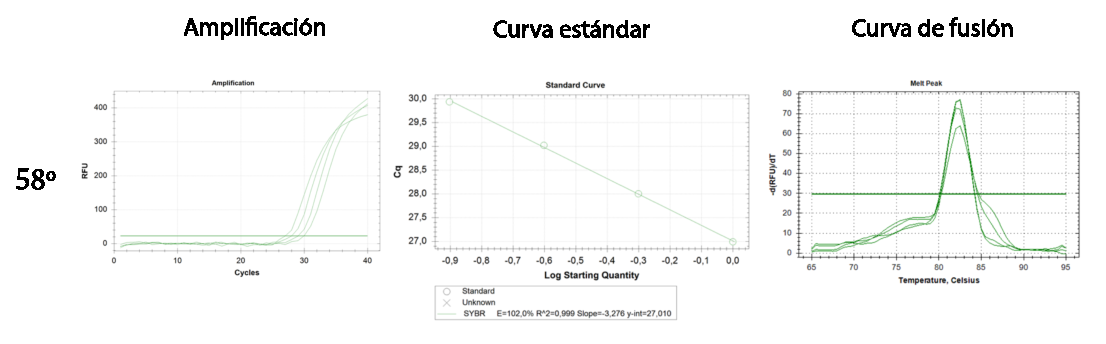
\includegraphics[width=0.9\textwidth]{peptidos/inos}
        \caption{iNOS}
        \label{fig:pep:inos}
    \end{subfigure}
    \begin{subfigure}{0.5\textwidth}
        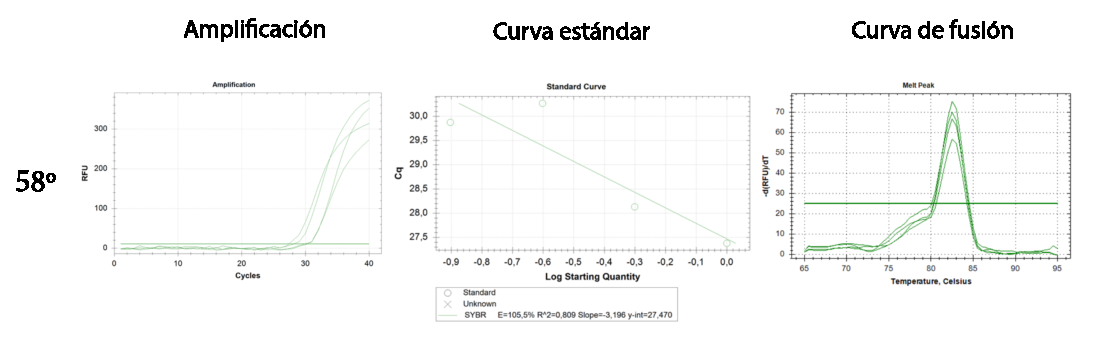
\includegraphics[width=0.9\textwidth]{peptidos/il12}
        \caption{IL-12}
        \label{fig:pep:il12}
    \end{subfigure}
    \caption{Evaluación cualitativa de los anticuerpos en estudio usando sus inmunógenos como antígenos, mediante ELISA Indirecto}
    \label{fig:pep}
\end{figure}

\subsection{Anticuerpos producidos en conejo}

Para el caso de los anticuerpos producidos en conejo,
anti-TNF-\(\alpha\) se obtuvo una curva con un \(R^2\) de 0,97 (Figura
\ref{fig:pep} \subref{fig:pep:tnfa}), el anticuerpo anti-IFN-\(\gamma\)
obtuvo una curva con un \(R^2\) de 0,9724(Figura \ref{fig:pep}
\subref{fig:pep:ifng}) y finalmente el anticuerpo anti-IL-1\(\beta\)
producido en conejo se obtuvo una curva con un \(R^2\) de 0,9859 (Figura
\ref{fig:pep} \subref{fig:pep:il1b}).

\subsection{Anticuerpos producidos en ratón}

En el caso de los anticuerpos producidos en murinos, anti-iNOS obtuvo
una curva con un \(R^2\) de 0,9934 (Figura \ref{fig:pep}
\subref{fig:pep:inos}) y para el anticuerpo anti-IL-12 se obtuvo un
\(R^2\) de 0,9753 (Figura \ref{fig:pep} \subref{fig:pep:il12}).

\section{ELISAs Indirectos}

Al evaluar mediante ELISA indirecto la presencia de las distintas
moleculas en estudio en las branquias de las truchas arcoiris
alimentadas con Zimosán A, se observó una clara diferencia entre los
individuos control y los tratados (Figura \ref{fig:elisa}).

\begin{figure}[h]
    \begin{subfigure}{0.5\textwidth}
        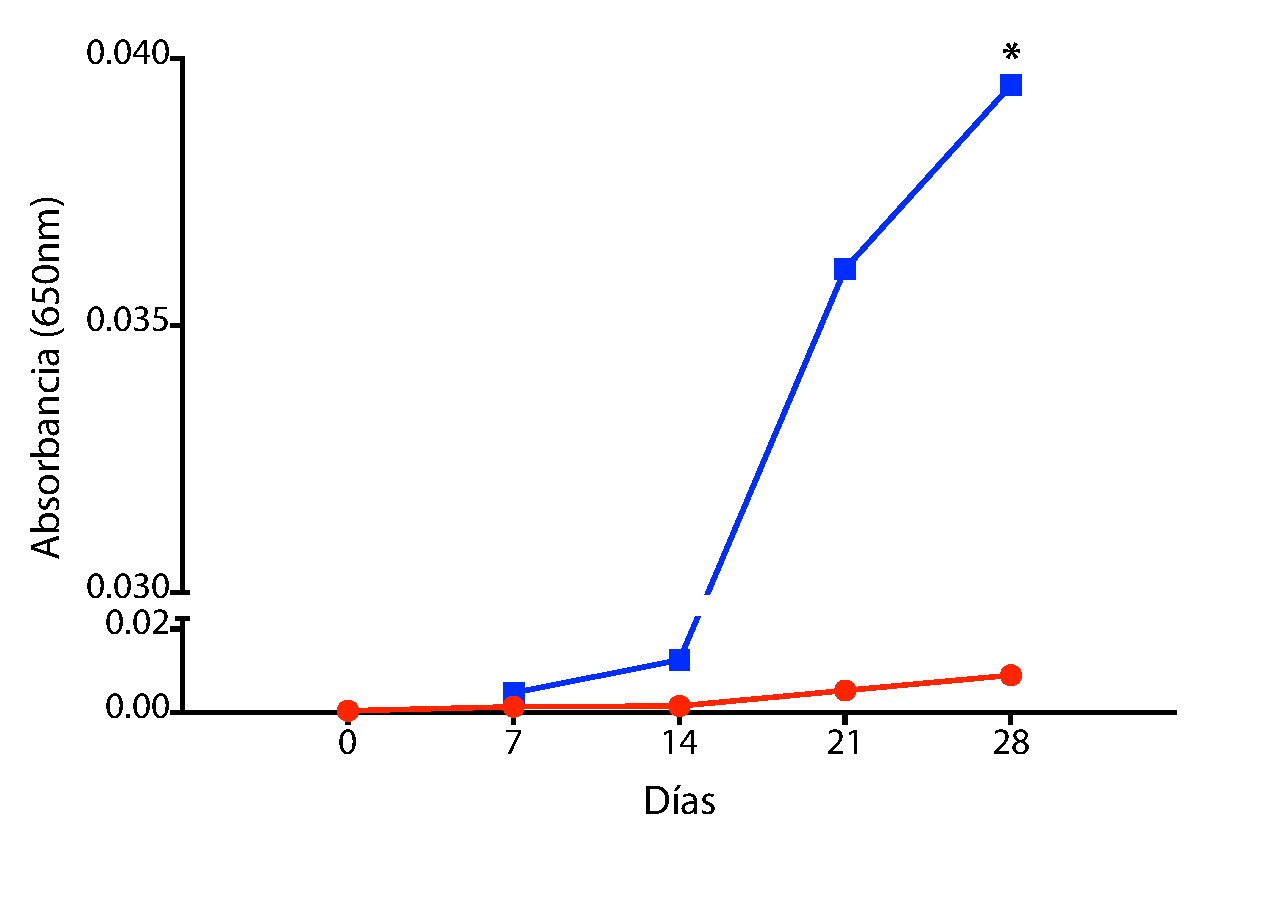
\includegraphics[width=0.9\textwidth]{eps/ELISA/etnfa}
        \caption{TNF-$\alpha$}
        \label{fig:elisa:tnfa}
        \end{subfigure}
    \begin{subfigure}{0.5\textwidth}
        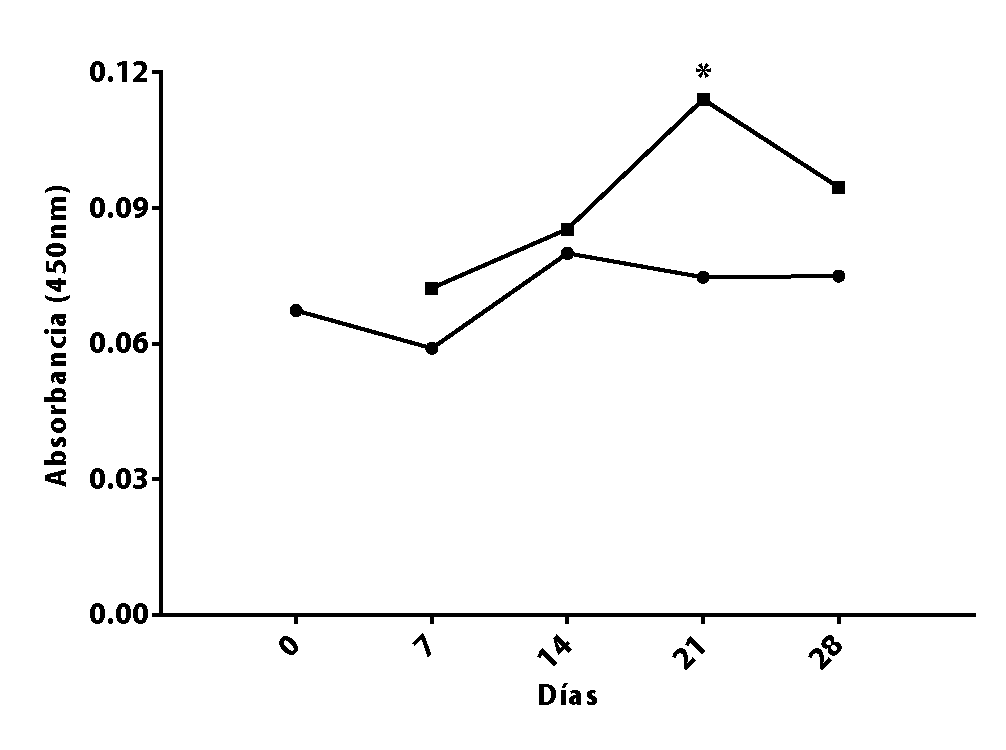
\includegraphics[width=0.9\textwidth]{eps/ELISA/eifng}
        \caption{IFN-$\gamma$}
        \label{fig:elisa:ifng}
    \end{subfigure}
    \end{figure}

\begin{figure}[h]
        \ContinuedFloat
    \begin{subfigure}{0.5\textwidth}
        \includegraphics[width=0.9\textwidth]{eps/ELISA/eil1b}
        \caption{IL-1$\beta$}
        \label{fig:elisa:il1b}
    \end{subfigure}
    \begin{subfigure}{0.5\textwidth}
        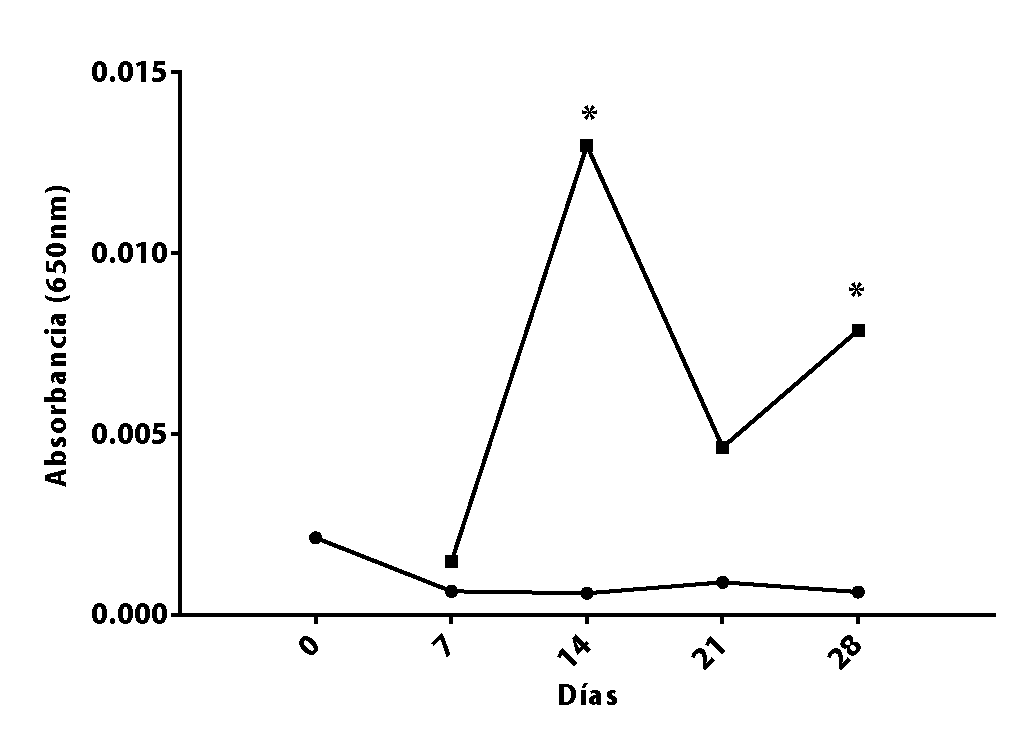
\includegraphics[width=0.9\textwidth]{eps/ELISA/einos}
        \caption{iNOS}
        \label{fig:elisa:inos}
    \end{subfigure}
    \begin{subfigure}{0.5\textwidth}
        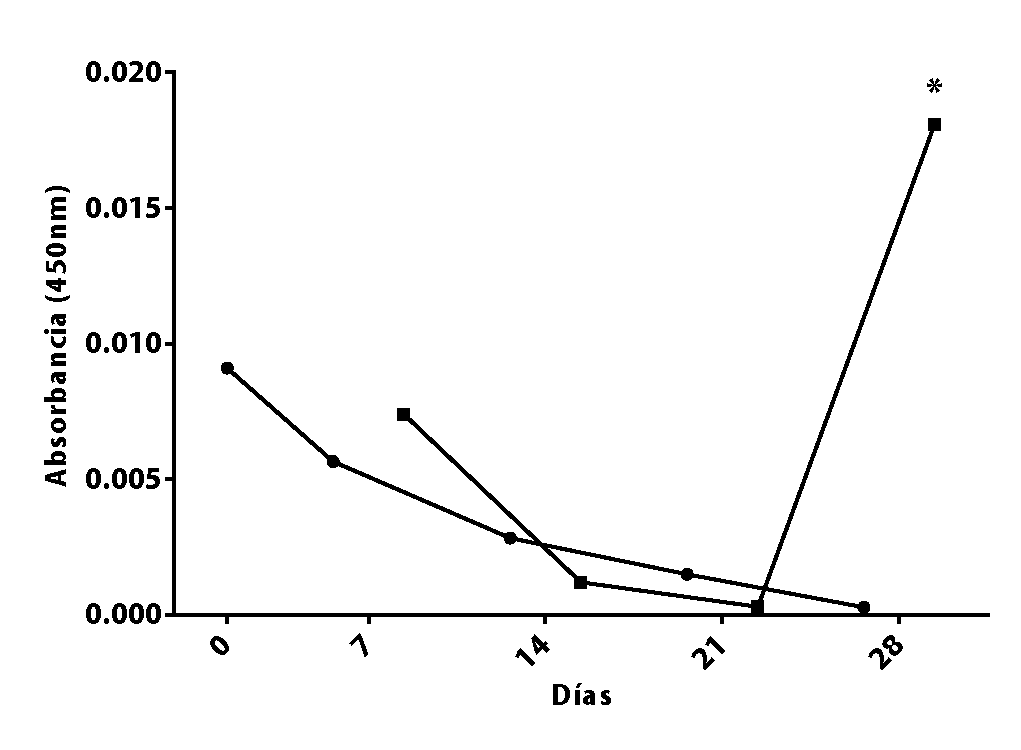
\includegraphics[width=0.9\textwidth]{eps/ELISA/eil12}
        \caption{IL-12}
        \label{fig:elisa:il12}
    \end{subfigure}
    \begin{subfigure}{0.5\textwidth}
        \includegraphics[width=0.9\textwidth]{eps/qPCR/leyenda}
    \end{subfigure}
    \caption{Detección mediante ELISA indirecto de las moléculas en estudio}
    \label{fig:elisa}
\end{figure}

\subsection{TNF-$\alpha$}

Para TNFa (Figura \ref{fig:elisa} \subref{fig:elisa:tnfa}), respecto a
su control inicial, evidenció un aumento paulatino de su
biodisponibilidad partiendo del dia 7 al día 14, un aumento de
aproximadamente 4 veces el día 21 y finalmente un leve aumento el día
28, este ultimo dia siendo significativo respecto a su control
(\(p \leq 0,05\)).

\subsection{IFN-$\gamma$}

Esta molécula (Figura \ref{fig:elisa} \subref{fig:elisa:ifng}) tuvo un
leve aumento en los dias 7 y 14 con respecto a su control,
evidenciandose el mayor aumento al día 21, el cual es significativo
(\(p \leq 0,05\)) con respecto a su control, para finalmente disminuir
su biodisponibilidad el día 28.

\subsection{IL-1$\beta$}

Para Interleuquina 1-\(\beta\) (Figura \ref{fig:elisa}
\subref{fig:elisa:il1b}) se observó una gran biodisponibilidad de esta
molécula en el control al inicio del tratamiento, pero esta alta
biodisponibilidad baja y se estabiliza rapidamente al día 7, en el caso
de los peces alimentados con Zimosán A se observaron desde el día 7
biodisponibilidades mayores a sus controles del día, siendo el dia 21 y
28 diferentes significativamente (\(p \leq 0,05\)).

\subsection{iNOS}

Para la enzima Oxido Nitrico Sintasa inducible (Figura \ref{fig:elisa}
\subref{fig:elisa:inos}) se obtuvo el dia 14 un súbito y significativo
aumento de su biodisponibilidad comparado con todo el grupo control
(\(p \leq 0,05\)), bajó el día 21 para finalmente subir paulatina y
signficativamente el día 28 con respecto a su control (\(p \leq 0,05\)).

\subsection{IL-12}

La Interleuquina 12 (Figura \ref{fig:elisa} \subref{fig:elisa:il12}) en
los peces tratados como los inducidos se obtuvo una baja en la
biodisponibilidad de esta molécula de los primeros 21 días, finalmente
después de esta medición, al día 28, hubo un aumento significativo de
aproximadamente 20 veces con respecto al control del día
(\(p \leq 0,05\)).

\clearpage

\section{Tinción Hematoxilina-eosina}

\begin{figure}[h!]
    \centering
    \fbox{\includegraphics{gills}}
    \caption[Microfotografías de branquias de trucha arcoiris]{Microfotografías de branquias de trucha arcoiris con tinción Hematoxilina-eosina: A) Operculo abierto exponiendo las branquias a extraer; B,C) Día 0; D) Día 14 Control; E) Día 14 Tratado; F) Día 21 Control; G) Día 21 Tratado; H) Día 28 Control; I) Día 28 Tratado. AB = Arco Branquial, B = Branquias, LP = Laminilla primaria, LS = Laminilla secundaria, CE = Células epiteliales CP = Células pilares}
    \label {fig:gills}
\end{figure}

Al realizar la tinción de Hematoxilina-eosina se pudo apreciar la
integridad de los distintos cortes histológicos, los tejidos que los
componen y asi como también los distintos tipos celulares que se
pudieron encontrar (Figura \ref{fig:gills}). La branquia se observa
completa, sin su arco branquial, demostrando una consistencia entre sus
laminillas primarias y secundarias (Figura \ref{fig:gills}D,E), así como
también la presencia de células pilares (Figura \ref{fig:gills}C) y
células epiteliales (Figura \ref{fig:gills}E).

\section{Inmunofluorescencia}

Habiendo comprobado la integridad de los tejidos muestreados se procedió
a localizar las moleculas en estudio, usando los cortes cortes
histológicos y la técnica de inmunofluorescencia descrita en
\ref{sec:ifat} se observaron los siguientes resultados.

\subsection{TNF-$\alpha$}

Se pueden observar al menos 5 marcajes correspondientes a celulas de la
laminilla secundaria las cuales mostraban producción de TNF-\(\alpha\)

\begin{figure}[h!]
    \centering
    \fbox{\includegraphics{ifat/tnfa}}
    \caption[Microscopía Confocal para TNF-$\alpha$]{Microscopía confocal para TNF-$\alpha$ en cortes histológicos de branquias de trucha arcoiris tratadas con Zimosán A liberado en dieta: A) Control con tinción Syto9; B) Control con tinción Alexa Fluor; C) \emph{Merge} entre ambos canales; D) Tratado con tinción Syto9; E) Tratado con tinción Alexa Fluor; F) \emph{Merge} entre ambos canales.  Flechas ($\leftarrow$) = Marcaje del anticuerpo}
    \label {fig:gills:tnfa}
\end{figure}

\subsection{IFNg-$\gamma$}

Se encontraron aproximadamente 4 marcajes correspondientes a celulas de
la laminilla secundaria, las cuales mostraban producción de interferón
gamma.

\begin{figure}[h!]
    \centering
    \fbox{\includegraphics{ifat/ifng}}
    \caption[Microscopía Confocal para IFN-$\gamma$]{Microscopía confocal para IFN-$\gamma$ en cortes histológicos de branquias de trucha arcoiris tratadas con Zimosán A liberado en dieta. Flechas ($\leftarrow$) = Marcaje del anticuerpo}
    \label {fig:gills:ifng}
\end{figure}

\subsection{IL-1$\beta$}

Se encontraron aproximadamente 3 marcajes correspondientes a celulas de
la laminilla secundaria, las cuales mostraban producción de
IL-1\(\beta\).

\begin{figure}[h!]
    \centering
    \fbox{\includegraphics{ifat/il1b}}
    \caption[Microscopía Confocal para IL-1$\beta$]{Microscopía confocal para IL-1$\beta$ en cortes histológicos de branquias de trucha arcoiris tratadas con Zimosán A liberado en dieta.  Flechas ($\leftarrow$) = Marcaje del anticuerpo}
    \label {fig:gills:il1b}
\end{figure}

\subsection{iNOS}

Al menos 2 marcajes se consideran positivos para la producción de iNOS
en celulas de la laminilla secundaria.

\begin{figure}[h!]
    \centering
    \fbox{\includegraphics{ifat/inos}}
    \caption[Microscopía Confocal para iNOS]{Microscopía confocal para iNOS en cortes histológicos de branquias de trucha arcoiris tratadas con Zimosán A liberado en dieta. Flechas ($\leftarrow$) = Marcaje del anticuerpo}
    \label {fig:gills:inos}
\end{figure}

\clearpage

\section{Correlación}

\begin{table}[h!]
\centering
\caption[Matrices de correlación de las moléculas en estudio]{Matrices de correlación de las moléculas en estudio, para qPCR y ELISA}\label{tab:corr}
\begin{subtable}{.5\textwidth}
\centering

\begin{tabular}{lrrrr}
\toprule
   & TNF-$\alpha$ & iNOS & IL-1$\beta$ & IL-12 \\ 
  \midrule
TNFa &  &  &  &  \\ 
  iNOS &  {\color{OliveGreen}0,81}  &  &  &  \\ 
  IL-1$\beta$ &  {\color{OliveGreen}0,98}  &  0,72  &  &  \\ 
  IL-12 &  {\color{OliveGreen}0,94}  &  {\color{OliveGreen}0,87}  &  {\color{OliveGreen}0,86}  &  \\ 
  IFN-$\gamma$ &  {\color{OliveGreen}0,99} &  {\color{OliveGreen}0,85}  &  {\color{OliveGreen}0,95}  &  {\color{OliveGreen}0,97}  \\ 
   \bottomrule
   \end{tabular}

\caption{qPCR}
\end{subtable}%
\begin{subtable}{.5\textwidth}
\centering

\begin{tabular}{lrrrr}
\toprule
        & TNF-$\alpha$ & iNOS & IL-1$\beta$ & IL-12 \\ 
  \midrule
  TNF-$\alpha$ & & & & \\
  iNOS &  0,31  &  &  &  \\ 
  IL-1$\beta$ & {\color{red}-0,81}  & -0,55  &  &  \\ 
  IL-12 &  0,20  & -0,15  & -0,02  &  \\ 
  IFN-$\gamma$ &  {\color{OliveGreen}0,89}  &  0,30  & -0,75  & -0,25  \\ 
   \bottomrule
   \end{tabular}

\caption{ELISA}
\end{subtable}
\end{table}

Se obtuvieron los coeficientes de correlación de Pearson, en los cuales
se obtuvo una correlación muy alta (\textgreater{}0.8) para el caso de
los ensayos de qPCR (Tabla \ref{tab:corr}A), siendo el mas alto la
correlación positiva para la dupla IFN-\(\gamma\)/TNF-\(\alpha\) con un
R=0,99 y por el contrario, la dupla con menor correlación positiva fue
IL-1\(\beta\)/iNOS.

En el caso de los ensayos de ELISA indirecto la dupla que obtuvo mayor
correlación positiva fue IFN-\(\gamma\)/TNF-\(\alpha\) con un R=0,89
mientras que para el caso de la dupla IL-1\(\beta\)/TNF-\(\alpha\) se
obtuvo una correlación negativa con un R=-0,82 (Tabla \ref{tab:corr}B).

Finalmente con el fin de saber que marcadores se pueden usar
indistintamente del ensayo que se ocupe (en este caso qPCR y ELISA) se
correlacionaron los datos obtenidos por cada molécula en cada ensayo.

\begin{table}[h!]
\centering
\begin{threeparttable}
\caption{Correlación de Pearson para una misma molécula y distintos ensayos}\label{r.pcr}\label{tab:corrtotal}
\begin{tabularx}{10cm}{X r}
  \toprule
    Dupla   &  R \\
  \midrule
qTNF-$\alpha$/eTNF-$\alpha$ & {\color{OliveGreen}0,96} \\
qIFN-$\gamma$/eIFN-$\gamma$ & {\color{OliveGreen}0,83} \\
qIL-12/eIL-12 & 0,52 \\
qiNOS/eiNOS & 0,02 \\
qIL-1$\beta$/eIL-1$\beta$ & 0,6 \\
 \bottomrule
   \end{tabularx}
   \begin{tablenotes}
    \item q = qPCR; e = ELISA
\end{tablenotes}
\end{threeparttable}
\end{table}

Para los casos de las moléculas TNF-\(\alpha\) e IFN-\(\gamma\) se
obtuvieron correlaciones positivas \textgreater{} a 0,8 (Tabla
\ref{tab:corrtotal}). \chapter{Discusiones}

La perdida del equilibrio
Ambiente\(\Leftrightarrow\)Patógeno\(\Leftrightarrow\)Hospedero es la
causa de la mayoria de las enfermedades presentes en la acuicultura, y
es por eso que es estrictamente necesario cimentar las bases de una
comprensión íntegra del sistema inmune, para así, poder generar
tecnología que pueda sobreponerse a estos paradigmas. Esto tiene suma
importancia sobretodo en la industria acuícola, la cual produce
anualmente, y con un crecimiento constante, 148 millones de toneladas de
pescado (FAO, 2012), las cuales se traducen aproximadamente en 217.500
millones de dolares (USD), mas aún, de toda esa producción, 128 millones
de toneladas fueron exclusivamente destinados a consumo humano, por lo
que las perdidas por un brote de alguna enfermedad ascienden a millones
de dolares, brotes que amenazan las año a año las operaciones acuicolas
al rededor del mundo.

\section{Objetivo 1}

Los inmunoestimulantes han surgido como una opción viable, escalable y
económica para solventar parte de los problemas de la acuicultura,
fortaleciendo su capacidad de respuesta inmune en distintos estadíos de
desarrollo. Dentro de las formas en las cuales se pueden desplegar estos
inmunoestimulantes podemos encontrar vacunas, suspensión oral y
liberación en el alimento, entre otras.

Para este proyecto se describió una dieta en base a \emph{pellets} de
harina de pescado, los cuales contenían como inmunoestimulante el
\(\beta\)-glucano \emph{Zimosán A}, proveniente de la levadura
\emph{Saccharomyces cerevisiae}, en una razón del 0,3\%.

Los peces se mantuvieron el CIAC alimentandose en dos grupos, control y
tratado, el totalidad de la mortalidad fue del 100\%, ya que todos los
peces se sacrificaron en los días determinado para ese fin dentro de la
linea de tiempo del ensayo.

Previo al desangramiento de cada pez se obtuvo el peso de cada
organismo, con el fin de confeccionar un grafico para evaluar si la
diferentes dietas generaban algun cambio en la masa del pez (Figura
\ref{fig:pesos}). Esto no fue así ya que el peso de ambos grupos se
mantuvo constante, los datos al ser correlacionados mediante el
coeficiente de Pearson obtuvieron un R = 0,962, lo que indica una
correlación positiva de casi un 100\%.

\section{Objetivo 2}

La extracción de RNA y su posterior cuantificación se mantuvo constante
(Tabla \ref{tablaRNA}), demostrando que en la mayoría de los casos se
trabajó prolijamente y sin mucha diferencia entre los distintos dias de
muestreo. Los dos unicos casos en que se obtuvo una concentración muy
baja fue en las muestras B2 y B41, con 63,3 y 40,20
\si{\nano\gramo}/\si{\micro\litro} respectivamente. Esto puede haberse
debido a una mala manipulacion del mortero, el cual alcanzaba
temperaturas cercanas a los -150ºC al mantenerse constantemente con
nitrógeno liquido,por lo tanto cuando se tomaba tejido pulverizado para
agregar al tubo de homogeneización se podría haber perdido algo de
muestra.

Con el RNA extraído y cuantificado se procedió a sintetizar su DNA
complementario, al haberse hecho esto con Kit y Termociclador salió todo
bien sin ninguna complicación, con lo que finalmente se pudo empezar a
realizar la estandarización de partidores.

El primer par de partidores en estandarizar fue el de referncia, el cual
tuvo una eficiencia de 96,9\% y solo un peak en la curva de disociación
lo que nos corrobora que el primer, a 58ºC como temperatura de
annealing, genera un solo producto y que cada ciclo dobla su cantidad
inicial de templado (Figura \ref{fig:ef1a}). Para las demas parejas de
partidores correspondientes a los genes en estudio se observó la misma
tendencia, generandose eficiencias de 105,5\% para el par de partidores
que amplifican para IL-12 a 58ºC (Figura \ref{fig:il12}), 115\% para el
el par de partidores que amplifican para TNF-\(\alpha\) a 58ºC (Figura
\ref{fig:tnfa}), 120,9\% para el par de partidores que amplifican para
IFN-\(\gamma\) a 61,5ºC (Figura \ref{fig:ifng}), 105,9\% para el par de
partidores que amplifican para IL-1\(\beta\) a 58ºC (Figure
\ref{fig:il1b}) y finalmente 102\% para la pareja de partidores que
amplifican para iNOS a 58ºC (Figura \ref{fig:inos}).

Todas las eficiencias son similares, la unica que se escapa un poco del
promedio es la eficiencia del par de partidores que amplifican para
IFN-\(\gamma\), esto puede deberse a que el producto o amplicón que
producen es muy pequeño (\textasciitilde{}51pb) (Tabla
\ref{tabla:partidores}) y está en el limite de lo recomendado para la
cuantificación por el metodo \(\Delta\Delta C_T\) (M. W. Pfaffl, 2001;
Bustin et~al., 2009).

Teniendo ya estandarizados todos los partidores se procedió a evaluar
las muestras biológicas del ensayo, en las cuales la tendencia demostró
que la respuesta inmune empieza a aumentar pasado el día 14, ya que
todos los peak de expresión se observaron en los días 21 y 28 según
corresponda. (Figura \ref{fig:qpcr}), esto se condice con varios
estudios donde los tiempos de respuesta frente a \(\beta\)-glucanos en
tratamientos \emph{in vivo} rondan dentro o después de los 21 días
(Casadei et~al., 2012; Skov et~al., 2012; Dobšíková et~al., 2013;
Morales-Lange et~al., 2014).

Para el caso de varios controles en distintas moleculas también se
observo un aumento pasado este día, esto puede deberse a un estrés en
los peces, el cual haya gatillado un aumento en la respuesta inmune como
se ha demostrado en estudios anteriores (Bricknell y Dalmo, 2005;
Magnadóttir, 2006; Barandica y Tort, 2008; Bowden, 2008), pero aún
teniendo controles altos en los ensayos de transcripción, por ejemplo
para TNF-\(\alpha\) (Figura \ref{fig:qpcr}A), IFN-\(\gamma\) (Figura
\ref{fig:qpcr}B) e IL-1\(\beta\) (Figura \ref{fig:qpcr}C) estas
diferencias entre tratamientos siguen siendo estadísticamente
significativas (\(p < 0,05\)).

Teniendo estos datos en cuenta se puede inferir que el suplementar la
alimentación de los peces con \emph{Zimosán A} liberado en dieta
promovería la expresión de los genes que codifican para distintas
citoquinas pro-inflamatorias y moléculas efectoras de inmunidad.

\section{Objetivo 3}

Para cuantificar las proteínas extraídas se utilizó el método BCA, en el
cual se obtuvo como resultado una curva de calibrado con un coeficiente
\(R^2 = 0,9976\) lo que indica que la recta es lineal y las
interpolaciones fueron válidas, esto así generando una cuantificación de
proteínas estable en todas las muestras (Tabla \ref{tablaPROTEINAS}),
demostrando a su vez la estandarización previa de los metodos usados en
el Laboratorio.

Los anticuerpos fueron a su vez validados usando ELISA indirecto,
obteniendo distintas curvas evaluando su reacción con su antígeno
correspondiente (Mason y Williams, 1980).

Para los 5 anticuerpos usados en el estudio se obtuvieron curvas
logarítmicas con un coeficiente \(R^2 > 0,97\), esto significa que a
mayor concentración de inmunógeno (péptido sintético) el anticuerpo se
va saturando, mientras que al inicio de la curva hay una linealidad en
la reacción. Con estos resultados se aprobó el uso de estos anticuerpos
en ensayos de ELISA indirectos con muestra biológica como antígeno.

Todas las moléculas en estudio aumentaron su biodisponibilidad con
respecto a sus controles. Tomando en cuenta el dogma de la biología
molecular debiese haber obtenido los peak de biodisponibilidad de
Proteínas posteriormente a los de transcrito, y hubieron casos, en que
hubo peaks al mismo día que en lo visto por PCR en tiempo real(Figuras
\ref{fig:elisa} y \ref{fig:qpcr}). Esto se puede deber a que exista un
intervalo de tiempo anterior al medido en que se pueda apreciar la
diferencia entre ambas condiciones y la biodisponibilidad de proteínas
que estamos observando corresponde a una traducción de transcrito de
algún día anterior no evaluado, y finalmente, otra razón de este
fenómeno sería la documentada presencia de leucocitos circulantes en las
branquias (Rosario Castro et~al., 2014) los cuales estarían produciendo
estas distintas moléculas reguladoras y efectoras de inmunidad.

Cabe destacar que la baja absorbancia obtenida en los ensayos se debe a
que el efecto del Zimosán A a esa concentración produce solo un leve
aumento en la respuesta inmune, lo cual está diseñado de esa forma, ya
que con este estudio tampoco se espera que haya un estallido
inflamatorio a nivel sistémico en el pez.

Sin embargo, a pesar de lo anteriormente mencionado, en los muestreos
posteriores al día 14 se aprecia un aumento notable en la
biodisponibilidad de todas las moléculas, con diferencias significativas
frente a sus controles, lo que corrobora lo visto a nivel de transcrito,
la liberación de Zimosán A en dieta genera una respuesta inmune
detectable a nivel de mRNA y proteínas.

Los resultados planteados en esta tesis sentarían las bases para
plantear que el receptor de \(\beta\)-glucanos descrito para
\emph{Salmo salar} (Guselle et~al., 2006; Morales-Lange et~al., 2014)
podría estar conservado dentro de la familia de los salmónidos.
\chapter{Conclusiones}

Los análisis desarrollados en esta tesis demuestran que al tratar a
\emph{O.mykiss} con \emph{Zimosan A} liberado en dieta, hay una
respuesta inmune en su tejido branquial, detectable y cuantificable a
nivel de transcrito y proteína, lo cual permite generar un modelo
molecular preliminar asociado a estos eventos (Figura \ref{fig:modelo}),
por lo cual se da por aceptada la hipótesis planteada en este trabajo.

Sintetizando:

\begin{itemize}
\item Se observa una respuesta inmune en tejido branquial de \emph{O.mykiss} al ser tratados con \emph{Zimosán A} liberado en dieta.
\item Esta respuesta es cuantificable y detectable a nivel de transcrito y proteínas.
\item Usando una concentración de 0,3\% de \emph{Zimosán A} esta respuesta puede ser detectada desde el día 21 de su tratamiento
\item Si bien los 5 marcadores propuestos en este ensayo, se sugiere utilizar específicamente (por su coeficiente de correlación de Pearson) TNF-$\alpha$ e IFN-$\gamma$, ya sea a nivel de transcrito o proteína
\item Los anticuerpos policlonales mono-específicos producidos por el Grupo de Marcadores Inmunológicos en Organismos Acuáticos del GIM-PUCV son una alternativa viable y económica para medir estos marcadores usando una pequeña cantidad de tejido.
\end{itemize}

El aumento de moléculas efectoras y reguladoras de inmunidad deben dotar
al pez de una mejor respuesta inmune frente a los distintos patógenos a
los que podrían estar enfrentados en el cultivo de esta especie.

Este trabajo sienta las bases concretas para que futuras investigaciones
se puedan centrar en el uso de \(\beta\)-glucanos, en especial
\emph{Zimosán A}, como inmunoestimulantes en distintas etapas de
crecimiento del pez, así como también la prueba de distintas
concentraciones y vías de liberación de estos compuestos.

\begin{figure}[h!]
\centering
    \includegraphics[width=0.8\textwidth]{modelo}
    \caption[Modelo molecular de respuesta inmune]{\textbf{Modelo molecular de respuesta inmune:} Generado a partir de los resultados obtenidos en tejido branquial de truchas arcoiris tratadas con \emph{Zimosán A} liberado en dieta, inmunoestimulante que llegaría a su receptor (¿$\beta$-glucano?, ¿Dectin-1 \emph{like}?), el cual generaría la cascada de señalización para promover una respuesta inmune sintetizando citoquinas como TNF-$\alpha$, IL-1$\beta$, IFN-$\gamma$ e IL-12 y a su vez promover un ambiente oxidativo con la síntesis de iNOS en células tipo NK}
    \label{fig:modelo}
\end{figure}

\chapter{Bibliografía}

Abarca, A. (2011). \emph{Implementación de un modelo in vitro para
determinar el poder inmunoestimulante de b-glucanos en macrofagos de
trucha arcoiris} (PhD thesis). Pontificia Universidad Catolica de
Valparaiso.

Abarca, A., Bethke, J., Narváez, E., Flores, R., \& Mercado, L. (2012).
Parameters to evaluate the immunostimulant effect of Zymosan A in head
kidney leucocytes ( HKL ) of salmonids Parámetros para la evaluación del
efecto de Zimosán A como inmunoestimulante sobre leucocitos de riñón
cefálico ( HKL ) de salmónidos, \emph{40}(3), 545-552.

Aghaallaei, N., Bajoghli, B., Schwarz, H., Schorpp, M., \& Boehm, T.
(2010). Characterization of mononuclear phagocytic cells in medaka fish
transgenic for a cxcr3a:gfp reporter. \emph{Proceedings of the National
Academy of Sciences of the United States of America}, \emph{107}(42),
18079-84.
doi:\href{http://dx.doi.org/10.1073/pnas.1000467107}{10.1073/pnas.1000467107}

Ainsworth, A. (1992). Fish granulocytes: Morphology, distribution, and
function. \emph{Annual Review of Fish Diseases}, \emph{2}, 123-148.
doi:\href{http://dx.doi.org/10.1016/0959-8030(92)90060-B}{10.1016/0959-8030(92)90060-B}

Alvarez-Pellitero, P. (2008). Fish immunity and parasite infections:
from innate immunity to immunoprophylactic prospects. \emph{Veterinary
immunology and immunopathology}, \emph{126}(3-4), 171-98.
doi:\href{http://dx.doi.org/10.1016/j.vetimm.2008.07.013}{10.1016/j.vetimm.2008.07.013}

Athman, R., \& Philpott, D. (2004). Innate immunity via Toll-like
receptors and Nod proteins. \emph{Current opinion in microbiology},
\emph{7}(1), 25-32.
doi:\href{http://dx.doi.org/10.1016/j.mib.2003.12.013}{10.1016/j.mib.2003.12.013}

Barandica, L., \& Tort, L. (2008). Neuroendocrinología e inmunologia de
la respuesta al estres en peces. \emph{Revista de la Academia Colombiana
de Ciencias Exactas, Físicas y Naturales}, \emph{32}(123), 267-284.
Recuperado a partir de
\url{http://www.accefyn.org.co/revista/Vol/_32/123/267-284.pdf}

Bengtén, E., Quiniou, S. M.-A., Stuge, T. B., Katagiri, T., Miller, N.
W., Clem, L. W., \ldots{} Wilson, M. (2002). The IgH Locus of the
Channel Catfish, Ictalurus punctatus, Contains Multiple Constant Region
Gene Sequences: Different Genes Encode Heavy Chains of Membrane and
Secreted IgD. \emph{The Journal of Immunology}, \emph{169}(5),
2488-2497. Recuperado a partir de
\url{http://jimmunol.org/content/169/5/2488.abstract}

Bethke, J., Rojas, V., Berendsen, J., Cárdenas, C., Guzmán, F.,
Gallardo, J. A., \& Mercado, L. (2012). Development of a new antibody
for detecting natural killer enhancing factor (NKEF)-like protein in
infected salmonids. \emph{Journal of fish diseases}, \emph{35}(5),
379-88.
doi:\href{http://dx.doi.org/10.1111/j.1365-2761.2012.01354.x}{10.1111/j.1365-2761.2012.01354.x}

Bilen, S., Bulut, M., \& Bilen, A. M. (2011). Immunostimulant effects of
Cotinus coggyria on rainbow trout (Oncorhynchus mykiss). \emph{Fish \&
shellfish immunology}, \emph{30}(2), 451-5.
doi:\href{http://dx.doi.org/10.1016/j.fsi.2010.12.013}{10.1016/j.fsi.2010.12.013}

Boehm, U., Klamp, T., Groot, M., \& Howard, J. C. (1997). Cellular
responses to interferon-gamma. \emph{Annual review of immunology},
\emph{15}, 749-95.
doi:\href{http://dx.doi.org/10.1146/annurev.immunol.15.1.749}{10.1146/annurev.immunol.15.1.749}

Bogdan, C. (2001). Nitric oxide and the immune response. \emph{Nature
immunology}, \emph{2}(10), 907-16.
doi:\href{http://dx.doi.org/10.1038/ni1001-907}{10.1038/ni1001-907}

Bols, N. C., Brubacher, J. L., Ganassin, R. C., \& Lee, L. E. (2001).
Ecotoxicology and innate immunity in fish. \emph{Developmental \&
Comparative Immunology}, \emph{25}(8-9), 853-873.
doi:\href{http://dx.doi.org/10.1016/S0145-305X(01)00040-4}{10.1016/S0145-305X(01)00040-4}

Boschi, I., Randelli, E., Buonocore, F., Casani, D., Bernini, C.,
Fausto, a M., \& Scapigliati, G. (2011). Transcription of T cell-related
genes in teleost fish, and the European sea bass (Dicentrarchus labrax)
as a model. \emph{Fish \& shellfish immunology}, \emph{31}(5), 655-62.
doi:\href{http://dx.doi.org/10.1016/j.fsi.2010.10.001}{10.1016/j.fsi.2010.10.001}

Bowden, T. J. (2008). Modulation of the immune system of fish by their
environment. \emph{Fish \& shellfish immunology}, \emph{25}(4), 373-83.
doi:\href{http://dx.doi.org/10.1016/j.fsi.2008.03.017}{10.1016/j.fsi.2008.03.017}

Bricknell, I., \& Dalmo, R. a. (2005). The use of immunostimulants in
fish larval aquaculture. \emph{Fish \& shellfish immunology},
\emph{19}(5), 457-72.
doi:\href{http://dx.doi.org/10.1016/j.fsi.2005.03.008}{10.1016/j.fsi.2005.03.008}

Bustin, S. a, Benes, V., Garson, J. a, Hellemans, J., Huggett, J.,
Kubista, M., \ldots{} Wittwer, C. T. (2009). The MIQE guidelines:
minimum information for publication of quantitative real-time PCR
experiments. \emph{Clinical chemistry}, \emph{55}(4), 611-22.
doi:\href{http://dx.doi.org/10.1373/clinchem.2008.112797}{10.1373/clinchem.2008.112797}

Casadei, E., Bird, S., González, J. L., Wadsworth, S., \& Secombes, C.
J. (2012). Fish \& Shell fi sh Immunology The effect of peptidoglycan
enriched diets on antimicrobial peptide gene expression in rainbow trout
( Oncorhynchus mykiss ). \emph{Fish and Shellfish Immunology},
(December), 1-9.
doi:\href{http://dx.doi.org/10.1016/j.fsi.2012.11.027}{10.1016/j.fsi.2012.11.027}

Castro, R., Bernard, D., Lefranc, M. P., Six, a, Benmansour, a, \&
Boudinot, P. (2011). T cell diversity and TcR repertoires in teleost
fish. \emph{Fish \& shellfish immunology}, \emph{31}(5), 644-54.
doi:\href{http://dx.doi.org/10.1016/j.fsi.2010.08.016}{10.1016/j.fsi.2010.08.016}

Castro, R., Bromage, E., Abós, B., Pignatelli, J., {González Granja},
A., Luque, A., \& Tafalla, C. (2014). CCR7 is mainly expressed in
teleost gills, where it defines an IgD+IgM- B lymphocyte subset.
\emph{Journal of immunology (Baltimore, Md. : 1950)}, \emph{192}(3),
1257-66.
doi:\href{http://dx.doi.org/10.4049/jimmunol.1302471}{10.4049/jimmunol.1302471}

Chang, C.-i., Pleguezuelos, O., Zhang, Y.-a., Zou, J., \& Secombes, C.
J. (2005). Identification of a novel cathelicidin gene in the rainbow
trout, Oncorhynchus mykiss. \emph{Infection and immunity}, \emph{73}(8),
5053-64.
doi:\href{http://dx.doi.org/10.1128/IAI.73.8.5053-5064.2005}{10.1128/IAI.73.8.5053-5064.2005}

Chang, C.-I., Zhang, Y.-A., Zou, J., Nie, P., \& Secombes, C. J. (2006).
Two cathelicidin genes are present in both rainbow trout (Oncorhynchus
mykiss) and atlantic salmon (Salmo salar). \emph{Antimicrobial agents
and chemotherapy}, \emph{50}(1), 185-95.
doi:\href{http://dx.doi.org/10.1128/AAC.50.1.185-195.2006}{10.1128/AAC.50.1.185-195.2006}

Chettri, J. K., Kania, P. W., \& Buchmann, K. (2013). Immunomodulation
of rainbow trout ( Oncorhynchus mykiss ) fry by bath exposure to a
\(\beta\)-glucan from Euglena gracilis. \emph{Aquaculture Research},
\emph{44}(9), 1407-1415.
doi:\href{http://dx.doi.org/10.1111/j.1365-2109.2012.03145.x}{10.1111/j.1365-2109.2012.03145.x}

Dalmo, R. a, \& Bøgwald, J. (2008). Beta-glucans as conductors of immune
symphonies. \emph{Fish \& shellfish immunology}, \emph{25}(4), 384-96.
doi:\href{http://dx.doi.org/10.1016/j.fsi.2008.04.008}{10.1016/j.fsi.2008.04.008}

Dobšíková, R., Blahová, J., Mikulíková, I., Modrá, H., Prášková, E.,
Svobodová, Z., \ldots{} Siwicki, A.-K. (2013). The effect of oyster
mushroom \(\beta\)-1.3/1.6-D-glucan and oxytetracycline antibiotic on
biometrical, haematological, biochemical, and immunological indices, and
histopathological changes in common carp (Cyprinus carpio L.).
\emph{Fish \& shellfish immunology}, \emph{35}(6), 1813-23.
doi:\href{http://dx.doi.org/10.1016/j.fsi.2013.09.006}{10.1016/j.fsi.2013.09.006}

Ellis, A. E. (1977). The leucocytes of fish: A review. \emph{Journal of
Fish Biology}, \emph{11}(5), 453-491.
doi:\href{http://dx.doi.org/10.1111/j.1095-8649.1977.tb04140.x}{10.1111/j.1095-8649.1977.tb04140.x}

Ellis, A. E. (2001). Innate host defense mechanisms of fish against
viruses and bacteria. \emph{Developmental and comparative immunology},
\emph{25}(8-9), 827-39. Recuperado a partir de
\url{http://www.ncbi.nlm.nih.gov/pubmed/11602198}

FAO. (2012). \emph{El estado mundial de la pesca y la acuicultura -
2012} (p. 251).

Fernández, A., Ruiz, I., \& Blas, I. D. (2002). El sistema inmune de los
teleósteos (I): Células y órganos. \emph{Revista AquaTIC}, \emph{16}.
Recuperado a partir de
\url{http://www.revistaaquatic.com/aquatic/html/art1605/inmune.htm}

Fields, B. N., Knipe, D. M., \& Howley, P. M. (2007). \emph{Fields'
Virology}. Wolters Kluwer Health/Lippincott Williams \& Wilkins.
Recuperado a partir de
\url{http://books.google.es/books?id=5O0somr0w18C}

Georgiadis, M., Gardner, I., \& Hedrick, R. (2001). The role of
epidemiology in the prevention, diagnosis, and control of infectious
diseases of fish. \emph{Preventive Veterinary Medicine}, \emph{48}(4),
287-302.
doi:\href{http://dx.doi.org/10.1016/S0167-5877(00)00202-6}{10.1016/S0167-5877(00)00202-6}

Gomez, D., Sunyer, J. O., \& Salinas, I. (2013). The mucosal immune
system of fish: the evolution of tolerating commensals while fighting
pathogens. \emph{Fish \& shellfish immunology}, \emph{35}(6), 1729-39.
doi:\href{http://dx.doi.org/10.1016/j.fsi.2013.09.032}{10.1016/j.fsi.2013.09.032}

Gordon, S. (2002). Pattern recognition receptors: doubling up for the
innate immune response. \emph{Cell}, \emph{111}(7), 927-30. Recuperado a
partir de \url{http://www.ncbi.nlm.nih.gov/pubmed/12507420}

Graves, S. S., Evans, D. L., Cobb, D., \& Dawe, D. L. (1984).
Nonspecific cytotoxic cells in fish (Ictalurus punctatus). I. Optimum
requirements for target cell lysis. \emph{Developmental and comparative
immunology}, \emph{8}(2), 293-302. Recuperado a partir de
\url{http://www.ncbi.nlm.nih.gov/pubmed/6734870}

Groot, C., \& Margolis, L. (1991). \emph{Pacific Salmon Life Histories}.
University of British Columbia Press. Recuperado a partir de
\url{http://books.google.es/books?id=I/_S0xCME0CYC}

Guselle, N. J., Markham, R. J. F., \& Speare, D. J. (2006). Short
communication to rainbow trout , Oncorhynchus mykiss ( Walbaum ),
protects against Loma salmonae, 375-381.

Hong, S., Zou, J., Collet, B., Bols, N. C., \& Secombes, C. J. (2004).
Analysis and characterisation of IL-1beta processing in rainbow trout,
Oncorhynchus mykiss. \emph{Fish \& shellfish immunology}, \emph{16}(3),
453-9.
doi:\href{http://dx.doi.org/10.1016/j.fsi.2003.08.002}{10.1016/j.fsi.2003.08.002}

Huising, M. O., Schijndel, J. E. van, Kruiswijk, C. P., Nabuurs, S. B.,
Savelkoul, H. F. J., Flik, G., \& {Verburg-van Kemenade}, B. M. L.
(2006). The presence of multiple and differentially regulated
interleukin-12p40 genes in bony fishes signifies an expansion of the
vertebrate heterodimeric cytokine family. \emph{Molecular immunology},
\emph{43}(10), 1519-33.
doi:\href{http://dx.doi.org/10.1016/j.molimm.2005.10.010}{10.1016/j.molimm.2005.10.010}

Kawai, T., \& Akira, S. (2005). Pathogen recognition with Toll-like
receptors. \emph{Current opinion in immunology}, \emph{17}(4), 338-44.
doi:\href{http://dx.doi.org/10.1016/j.coi.2005.02.007}{10.1016/j.coi.2005.02.007}

Kumari, J., \& Sahoo, P. K. (2006). Dietary immunostimulants influence
specific immune response and resistance of healthy and immunocompromised
Asian catfish Clarias batrachus to Aeromonas hydrophila infection.
\emph{Diseases of aquatic organisms}, \emph{70}(1-2), 63-70.
doi:\href{http://dx.doi.org/10.3354/dao070063}{10.3354/dao070063}

Kühlwein, H., Merrifield, D. L., Rawling, M. D., Foey, a D., \& Davies,
S. J. (2014). Effects of dietary \(\beta\)-(1,3)(1,6)-D-glucan
supplementation on growth performance, intestinal morphology and
haemato-immunological profile of mirror carp (Cyprinus carpio L.).
\emph{Journal of animal physiology and animal nutrition}, \emph{98}(2),
279-89.
doi:\href{http://dx.doi.org/10.1111/jpn.12078}{10.1111/jpn.12078}

Lazado, C. C., \& Caipang, C. M. A. (2014). Mucosal immunity and
probiotics in fish. \emph{Fish \& shellfish immunology}, \emph{39}(1),
78-89.
doi:\href{http://dx.doi.org/10.1016/j.fsi.2014.04.015}{10.1016/j.fsi.2014.04.015}

Lin, S., Pan, Y., Luo, L., \& Luo, L. (2011). Effects of dietary
\(\beta\)-1,3-glucan, chitosan or raffinose on the growth, innate
immunity and resistance of koi (Cyprinus carpio koi). \emph{Fish \&
shellfish immunology}, \emph{31}(6), 788-94.
doi:\href{http://dx.doi.org/10.1016/j.fsi.2011.07.013}{10.1016/j.fsi.2011.07.013}

Lokesh, J., Fernandes, J. M. O., Korsnes, K., Bergh, O., Brinchmann, M.
F., \& Kiron, V. (2012). Transcriptional regulation of cytokines in the
intestine of Atlantic cod fed yeast derived mannan oligosaccharide or
\(\beta\)-glucan and challenged with Vibrio anguillarum. \emph{Fish \&
shellfish immunology}, \emph{33}(3), 626-31.
doi:\href{http://dx.doi.org/10.1016/j.fsi.2012.06.017}{10.1016/j.fsi.2012.06.017}

MacMicking, J., Xie, Q. W., \& Nathan, C. (1997). Nitric oxide and
macrophage function. \emph{Annual review of immunology}, \emph{15},
323-50.
doi:\href{http://dx.doi.org/10.1146/annurev.immunol.15.1.323}{10.1146/annurev.immunol.15.1.323}

Magnadóttir, B. (2006). Innate immunity of fish (overview). \emph{Fish
\& shellfish immunology}, \emph{20}(2), 137-51.
doi:\href{http://dx.doi.org/10.1016/j.fsi.2004.09.006}{10.1016/j.fsi.2004.09.006}

Maier, V. H., Dorn, K. V., Gudmundsdottir, B. K., \& Gudmundsson, G. H.
(2008). Characterisation of cathelicidin gene family members in
divergent fish species. \emph{Molecular immunology}, \emph{45}(14),
3723-30.
doi:\href{http://dx.doi.org/10.1016/j.molimm.2008.06.002}{10.1016/j.molimm.2008.06.002}

Mason, D. W., \& Williams, A. F. (1980). The kinetics of antibody
binding to membrane antigens in solution and at the cell surface.
\emph{The Biochemical journal}, \emph{187}(1), 1-20. Recuperado a partir
de
\url{http://www.pubmedcentral.nih.gov/articlerender.fcgi?artid=1162489/\&tool=pmcentrez/\&rendertype=abstract}

Mercado, L., Schmitt, P., Marshall, S. H., \& Arenas, G. (2005). Gill
tissues of the mussel Mytilus edulis chilensis: A new source for
antimicrobial peptides. \emph{Electronic Journal of Biotechnology},
\emph{8}(3), 284-290.
doi:\href{http://dx.doi.org/10.2225/vol8-issue3-fulltext-2}{10.2225/vol8-issue3-fulltext-2}

Morales-Lange, B., Bethke, J., Schmitt, P., \& Mercado, L. (2014).
Phenotypical parameters as a tool to evaluate the immunostimulatory
effects of laminarin in Oncorhynchus mykiss. \emph{Aquaculture
Research}, n/a-n/a.
doi:\href{http://dx.doi.org/10.1111/are.12426}{10.1111/are.12426}

Mulero, I., {Pilar Sepulcre}, M., Roca, F. J., Meseguer, J.,
García-Ayala, A., \& Mulero, V. (2008). Characterization of macrophages
from the bony fish gilthead seabream using an antibody against the
macrophage colony-stimulating factor receptor. \emph{Developmental and
comparative immunology}, \emph{32}(10), 1151-9.
doi:\href{http://dx.doi.org/10.1016/j.dci.2008.03.005}{10.1016/j.dci.2008.03.005}

Narváez, E., Berendsen, J., Guzmán, F., Gallardo, J. a, \& Mercado, L.
(2010). An immunological method for quantifying antibacterial activity
in Salmo salar (Linnaeus, 1758) skin mucus. \emph{Fish \& shellfish
immunology}, \emph{28}(1), 235-9.
doi:\href{http://dx.doi.org/10.1016/j.fsi.2009.10.004}{10.1016/j.fsi.2009.10.004}

Nascimento, D. S., Vale, A. do, Tomás, A. M., Zou, J., Secombes, C. J.,
\& Santos, N. M. S. dos. (2007). Cloning, promoter analysis and
expression in response to bacterial exposure of sea bass (Dicentrarchus
labrax L.) interleukin-12 p40 and p35 subunits. \emph{Molecular
immunology}, \emph{44}(9), 2277-91.
doi:\href{http://dx.doi.org/10.1016/j.molimm.2006.11.006}{10.1016/j.molimm.2006.11.006}

Oikawa, B. Y. S., \& Itazawa, Y. (1985). Gill and Body Surface Areas of
the Carp in relation to Body Mass, With Special Reference To The
Metabolism-Size Relationship. \emph{The Journal of experimental
biology}, \emph{14}(117), 1-14.

Olabuenaga, S. E. (2000). Sistema inmune en peces. \emph{Gayana
(Concepción)}, \emph{64}(2).
doi:\href{http://dx.doi.org/10.4067/S0717-65382000000200010}{10.4067/S0717-65382000000200010}

Palić, D., Beck, L. S., Palić, J., \& Andreasen, C. B. (2011). Use of
rapid cytochemical staining to characterize fish blood granulocytes in
species of special concern and determine potential for function testing.
\emph{Fish \& shellfish immunology}, \emph{30}(2), 646-52.
doi:\href{http://dx.doi.org/10.1016/j.fsi.2010.12.024}{10.1016/j.fsi.2010.12.024}

Peddie, S., Zou, J., \& Secombes, C. J. (2002). Immunostimulation in the
rainbow trout (Oncorhynchus mykiss) following intraperitoneal
administration of Ergosan. \emph{Veterinary Immunology and
Immunopathology}, \emph{86}(1-2), 101-113.
doi:\href{http://dx.doi.org/10.1016/S0165-2427(02)00019-3}{10.1016/S0165-2427(02)00019-3}

Pfaffl, M. W. (2001). A new mathematical model for relative
quantification in real-time RT-PCR. \emph{Nucleic acids research},
\emph{29}(9), e45. Recuperado a partir de
\href{http://www.ncbi.nlm.nih.gov/pubmed/55695 http://www.pubmedcentral.nih.gov/articlerender.fcgi?artid=55695/\&tool=pmcentrez/\&rendertype=abstract}{http://www.ncbi.nlm.nih.gov/pubmed/55695 http://www.pubmedcentral.nih.gov/articlerender.fcgi?artid=55695\textbackslash{}\&tool=pmcentrez\textbackslash{}\&rendertype=abstract}

Razquin, B. E., Castillo, A., Lopez-Fierro, P., Alvarez, F., Zapata, A.,
\& Villena, A. J. (1990). Ontogeny of IgM-producing cells in the
lymphoid organs of rainbow trout, Salmo gairdneri Richardson: an immuno-
and enzyme-histochemical study. \emph{Journal of Fish Biology},
\emph{36}(2), 159-173.
doi:\href{http://dx.doi.org/10.1111/j.1095-8649.1990.tb05592.x}{10.1111/j.1095-8649.1990.tb05592.x}

Reis, M. I. R., Vale, A. do, Pereira, P. J. B., Azevedo, J. E., \& {Dos
Santos}, N. M. S. (2012). Caspase-1 and IL-1\(\beta\) processing in a
teleost fish. \emph{PloS one}, \emph{7}(11), e50450.
doi:\href{http://dx.doi.org/10.1371/journal.pone.0050450}{10.1371/journal.pone.0050450}

Rodríguez, I., Chamorro, R., Novoa, B., \& Figueras, A. (2009).
beta-Glucan administration enhances disease resistance and some innate
immune responses in zebrafish (Danio rerio). \emph{Fish \& shellfish
immunology}, \emph{27}(2), 369-73.
doi:\href{http://dx.doi.org/10.1016/j.fsi.2009.02.007}{10.1016/j.fsi.2009.02.007}

Rojas, V., Guzman, F., \& Morales-lange, B. (2012). Immunological
strategy for detecting the pro-inflammatory cytokine TNF-alpha in
salmonids. \emph{Electronic Journal of Biotechnology}, \emph{15}.
doi:\href{http://dx.doi.org/10.2225/vol15-issue5-fulltext-19}{10.2225/vol15-issue5-fulltext-19}

Rombout, J. H. W. M., Abelli, L., Picchietti, S., Scapigliati, G., \&
Kiron, V. (2011). Teleost intestinal immunology. \emph{Fish \& shellfish
immunology}, \emph{31}(5), 616-26.
doi:\href{http://dx.doi.org/10.1016/j.fsi.2010.09.001}{10.1016/j.fsi.2010.09.001}

Rondon-Barragan, I. (2010). Receptores similares a Toll en peces : el
inicio de la divergencia. \emph{Investigación Veterinaria},
\emph{11}(1), 15-30.

Salazar-Mather, T., \& Hokeness, K. (2006). Cytokine and Chemokine
Networks: Pathways to Antiviral Defense. En T. E. Lane (ed.),
\emph{Chemokines and viral infection} (Vol. 303, pp. 29-46). Springer
Berlin Heidelberg. Recuperado a partir de
\url{http://dx.doi.org/10.1007/978-3-540-33397-5/_2}

Salinas, I., Zhang, Y.-A., \& Sunyer, J. O. (2011). Mucosal
immunoglobulins and B cells of teleost fish. \emph{Developmental and
comparative immunology}, \emph{35}(12), 1346-65.
doi:\href{http://dx.doi.org/10.1016/j.dci.2011.11.009}{10.1016/j.dci.2011.11.009}

Santana, P., Palacios, C., Narváez, E., \& Guzmán, F. (2012).
Anti-peptide antibodies : A tool for detecting IL-8 in salmonids,
\emph{15}.
doi:\href{http://dx.doi.org/10.2225/vol15-issue5-fulltext-15}{10.2225/vol15-issue5-fulltext-15}

Santos, N. M. dos, Taverne-Thiele, J. J., Barnes, A. C., Muiswinkel, W.
B. van, Ellis, A. E., \& Rombout, J. H. (2001). The gill is a major
organ for antibody secreting cell production following direct immersion
of sea bass (Dicentrarchus labrax, L.) in a Photobacterium damselae ssp.
piscicida bacterin: an ontogenetic study. \emph{Fish \& shellfish
immunology}, \emph{11}(1), 65-74.
doi:\href{http://dx.doi.org/10.1006/fsim.2000.0295}{10.1006/fsim.2000.0295}

Savan, R., \& Sakai, M. (2006). Genomics of fish cytokines.
\emph{Comparative biochemistry and physiology. Part D, Genomics \&
proteomics}, \emph{1}(1), 89-101.
doi:\href{http://dx.doi.org/10.1016/j.cbd.2005.08.005}{10.1016/j.cbd.2005.08.005}

Scapigliati, G., Romano, N., \& Abelli, L. (1999). Monoclonal antibodies
in fish immunology : identification , ontogeny and activity of T- and
B-lymphocytes. \emph{Aquaculture}, \emph{172}, 3-28.

Secombes, C. J., Wang, T., \& Bird, S. (2011). The interleukins of fish.
\emph{Developmental and comparative immunology}, \emph{35}(12), 1336-45.
doi:\href{http://dx.doi.org/10.1016/j.dci.2011.05.001}{10.1016/j.dci.2011.05.001}

Sernapesca. (2012). Anuario desembarques. Santiago de Chile: Gobierno de
Chile. Recuperado a partir de \url{http://www.sernapesca.cl}

Shao, Z. J. (2001). Aquaculture pharmaceuticals and biologicals: current
perspectives and future possibilities. \emph{Advanced Drug Delivery
Reviews}, \emph{50}(3), 229-243.
doi:\href{http://dx.doi.org/10.1016/S0169-409X(01)00159-4}{10.1016/S0169-409X(01)00159-4}

Sharpey-Schäfer, E. A., \& Carleton, H. M. (1938). Schafer's essentials
of histology: descriptive and practical for the use of students. London
; New York: Longmans, Green. Recuperado a partir de
\href{http://catalog.hathitrust.org/Record/009241076 http://hdl.handle.net/2027/uc1./\$b439719}{http://catalog.hathitrust.org/Record/009241076 http://hdl.handle.net/2027/uc1.\textbackslash{}\$b439719}

Skov, J., Kania, P. W., Holten-Andersen, L., Fouz, B., \& Buchmann, K.
(2012). Immunomodulatory effects of dietary \(\beta\)-1,3-glucan from
Euglena gracilis in rainbow trout (Oncorhynchus mykiss) immersion
vaccinated against Yersinia ruckeri. \emph{Fish \& shellfish
immunology}, \emph{33}(1), 111-20.
doi:\href{http://dx.doi.org/10.1016/j.fsi.2012.04.009}{10.1016/j.fsi.2012.04.009}

Smith, P. K., Krohn, R. I., Hermanson, G. T., Mallia, A. K., Gartner, F.
H., Provenzano, M. D., \ldots{} Klenk, D. C. (1985). Measurement of
protein using bicinchoninic acid. \emph{Analytical biochemistry},
\emph{150}(1), 76-85. Recuperado a partir de
\url{http://www.ncbi.nlm.nih.gov/pubmed/3843705}

Subpesca. (2013). Cuenta Pública de Estado de los Recursos. Santiago de
Chile: Gobierno de Chile. Recuperado a partir de
\url{http://www.subpesca.cl}

Taechavasonyoo, A., Kondo, H., Nozaki, R., Suzuki, Y., \& Hirono, I.
(2013). Identification of novel interleukin 1 beta family genes in
Japanese flounder Paralichthys olivaceus. \emph{Fish \& shellfish
immunology}, \emph{34}(1), 393-6.
doi:\href{http://dx.doi.org/10.1016/j.fsi.2012.10.001}{10.1016/j.fsi.2012.10.001}

Teles, M., Mackenzie, S., Boltaña, S., Callol, a, \& Tort, L. (2011).
Gene expression and TNF-alpha secretion profile in rainbow trout
macrophages following exposures to copper and bacterial
lipopolysaccharide. \emph{Fish \& shellfish immunology}, \emph{30}(1),
340-6.
doi:\href{http://dx.doi.org/10.1016/j.fsi.2010.11.006}{10.1016/j.fsi.2010.11.006}

Volman, J. J., Ramakers, J. D., \& Plat, J. (2008). Dietary modulation
of immune function by beta-glucans. \emph{Physiology \& behavior},
\emph{94}(2), 276-84.
doi:\href{http://dx.doi.org/10.1016/j.physbeh.2007.11.045}{10.1016/j.physbeh.2007.11.045}

Wang, T., Johnson, N., Zou, J., Bols, N., \& Secombes, C. J. (2004).
Sequencing and expression of the second allele of the interleukin-1beta1
gene in rainbow trout (Oncorhynchus mykiss): identification of a novel
SINE in the third intron. \emph{Fish \& shellfish immunology},
\emph{16}(3), 335-58.
doi:\href{http://dx.doi.org/10.1016/S1050-4648(03)00114-1}{10.1016/S1050-4648(03)00114-1}

Wang, W.-S., Hung, S.-W., Lin, Y.-H., Tu, C.-Y., Wong, M.-L., Chiou,
S.-H., \& Shieh, M.-T. (2007). The effects of five different glycans on
innate immune responses by phagocytes of hybrid tilapia and Japanese
eels Anguilla japonica. \emph{Journal of aquatic animal health},
\emph{19}(1), 49-59.
doi:\href{http://dx.doi.org/10.1577/H06-020.1}{10.1577/H06-020.1}

Whyte, S. K. (2007). The innate immune response of finfish--a review of
current knowledge. \emph{Fish \& shellfish immunology}, \emph{23}(6),
1127-51.
doi:\href{http://dx.doi.org/10.1016/j.fsi.2007.06.005}{10.1016/j.fsi.2007.06.005}

Wilson, J. M., \& Laurent, P. (2002). Fish gill morphology: inside out.
\emph{The Journal of experimental zoology}, \emph{293}(3), 192-213.
doi:\href{http://dx.doi.org/10.1002/jez.10124}{10.1002/jez.10124}

Wimley, W. C. (2010). Describing the mechanism of antimicrobial peptide
action with the interfacial activity model. \emph{ACS chemical biology},
\emph{5}(10), 905-17.
doi:\href{http://dx.doi.org/10.1021/cb1001558}{10.1021/cb1001558}

Wittwer, C. T., Herrmann, M. G., Moss, A. a, \& Rasmussen, R. P. (1997).
Continuous fluorescence monitoring of rapid cycle DNA amplification.
1997. \emph{BioTechniques}, \emph{54}(6), 314-20. Recuperado a partir de
\url{http://www.ncbi.nlm.nih.gov/pubmed/23905170}

Wu, F., Tyml, K., \& Wilson, J. X. (2008). iNOS expression requires
NADPH oxidase-dependent redox signaling in microvascular endothelial
cells. \emph{Journal of cellular physiology}, \emph{217}(1), 207-14.
doi:\href{http://dx.doi.org/10.1002/jcp.21495}{10.1002/jcp.21495}

Yang, K., Zhang, S., Chen, D., Zhang, A., Wang, X., \& Zhou, H. (2013).
IFN-\(\gamma\)-activated lymphocytes boost nitric oxide production in
grass carp monocytes/macrophages. \emph{Fish \& shellfish immunology},
\emph{35}(5), 1635-41.
doi:\href{http://dx.doi.org/10.1016/j.fsi.2013.09.017}{10.1016/j.fsi.2013.09.017}

Yoshiura, Y., Kiryu, I., Fujiwara, A., Suetake, H., Suzuki, Y.,
Nakanishi, T., \& Ototake, M. (2003). Identification and
characterization of Fugu orthologues of mammalian interleukin-12
subunits. \emph{Immunogenetics}, \emph{55}(5), 296-306.
doi:\href{http://dx.doi.org/10.1007/s00251-003-0582-9}{10.1007/s00251-003-0582-9}

Zasloff, M. (2002). Antimicrobial peptides of multicellular organisms.
\emph{Nature}, \emph{415}(6870), 389-95.
doi:\href{http://dx.doi.org/10.1038/415389a}{10.1038/415389a}

Zhang, L., Li, Y.-y., Chen, T., Xia, W., Zhou, Y., Wan, Y.-j., \ldots{}
Xu, S.-q. (2011). Abnormal development of motor neurons in
perfluorooctane sulphonate exposed zebrafish embryos.
\emph{Ecotoxicology (London, England)}, \emph{20}(4), 643-52.
doi:\href{http://dx.doi.org/10.1007/s10646-011-0604-6}{10.1007/s10646-011-0604-6}

Zhang, L., Zhang, B.-C., \& Hu, Y.-H. (2014). Rock bream (Oplegnathus
fasciatus) IL-12p40: identification, expression, and effect on bacterial
infection. \emph{Fish \& shellfish immunology}.
doi:\href{http://dx.doi.org/10.1016/j.fsi.2014.05.026}{10.1016/j.fsi.2014.05.026}

Zhang, Z., Swain, T., Bøgwald, J., Dalmo, R. a, \& Kumari, J. (2009).
Bath immunostimulation of rainbow trout (Oncorhynchus mykiss) fry
induces enhancement of inflammatory cytokine transcripts, while repeated
bath induce no changes. \emph{Fish \& shellfish immunology},
\emph{26}(5), 677-84.
doi:\href{http://dx.doi.org/10.1016/j.fsi.2009.02.014}{10.1016/j.fsi.2009.02.014}

Zhao, K., Huang, Z., Lu, H., Zhou, J., \& Wei, T. (2010). Induction of
inducible nitric oxide synthase increases the production of reactive
oxygen species in RAW264.7 macrophages. \emph{Bioscience reports},
\emph{30}(4), 233-41.
doi:\href{http://dx.doi.org/10.1042/BSR20090048}{10.1042/BSR20090048}

Zhu, L.-Y., Nie, L., Zhu, G., Xiang, L.-X., \& Shao, J.-Z. (2012).
Advances in research of fish immune-relevant genes: A comparative
overview of innate and adaptive immunity in teleosts.
\emph{Developmental and comparative immunology}.
doi:\href{http://dx.doi.org/10.1016/j.dci.2012.04.001}{10.1016/j.dci.2012.04.001}

Zou, J., Peddie, S., Scapigliati, G., Zhang, Y., Bols, N., Ellis, \&
Secombes, C. (2003). Functional characterisation of the recombinant
tumor necrosis factors in rainbow trout, Oncorhynchus mykiss.
\emph{Developmental \& Comparative Immunology}, \emph{27}(9), 813-822.
doi:\href{http://dx.doi.org/10.1016/S0145-305X(03)00077-6}{10.1016/S0145-305X(03)00077-6}

\end{document}
